% !TeX root = main.tex
\chapter{Paper-based semantic speech editing}\label{chp:paper}

% Need for paper
One of the findings from Chapter~\ref{chp:screen} was that some producers find their work environment noisy and
distracting, and do not like working with screens for extended periods. This leads many to print out transcripts of
speech recordings so that they can review and edit the recordings away from the screen and/or office.

% Advantage of paper
Working on paper offers a number of advantages over working on screens. Most of these are self-evident, but still
worth reviewing.  Paper is lightweight, portable and does not require any power, which allows users to work almost
anywhere.  It is not back-lit, so is easier on the eyes.  It can be navigated quickly, annotated freely whilst reading,
and individual pages can be laid out and easily compared.  Its physical low-tech nature also means that it is
intuitive, robust, durable and does not crash or lose data.  Reading from paper rather than a screen allows readers to
gain a deeper understanding, easily cross-reference other documents, and interleave reading and writing
\citep{OHara1997,Mangen2013,Singer2017}.

%Transcripts are often printed out because:
%- it is easier to read than on screen
%- allows portability,
%- allows annotation,
%- flexible spatial layout
%- quick navigation
%- cross-referencing,
%- reduces battery anxiety,
%- more trusted by non-tech-savvy users

%A similar process happens in the production of media content. The production workflow typically involves recording
%material, selecting which parts of that material to use, then editing the desired material down to the final output
%\citep{Baume2015}.  Many producers will `log' the material after it is recorded by writing transcripts of what was
%said.  This is either done themselves or using a third-party service. These transcripts help producers to recall what
%was said and when, identify themes, and make links between different parts of their content.

% Disadvantage of paper
Compared to digital media, working with a physical medium like paper introduces restrictions that make it more
difficult to copy, share, store and archive information. Printing a document breaks the link to its digital source, so
is normally a one-way process, where any information that is changed/added cannot is not fed back. Additionally,
freehand annotations are unstructured, and cannot easily be digitised and re-used. This forces users to manually
re-enter the information into a computer. In the case of radio production, this involves using a DAW to edit the audio
based on paper notes, which can be slow and tedious.

% Digital paper
There are a number of technological solutions that can be used to create a `digital bridge' between paper and
its digital source. These offer the possibility to combine the advantages of paper and digital workflows. Using this
approach, it is possible to link the words on a printed transcript of speech to the time they were spoken in the
original audio recording. Furthermore, by linking the paper annotations to audio edit commands, the paper could be used
to directly edit the audio content.

% Intro
In this chapter, we investigate paper-based workflows in the context of professional radio production. We describe how
we captured the requirements for a paper-based speech editor, and how we designed and built a working prototype. We
then describe a contextual study of radio production in which we directly compared screen-based and paper-based
workflows. 

\section{Background}\label{sec:paper-background}
Radio production using a paper interface requires a system that automatically translates annotations on a printed
transcript to audio edit commands. Such a system requires a method of linking paper to media.

`The Audio Notebook' \citep{Stifelman2001} was a system that used a physical pen and paper interface in combination
with a device that recorded audio synchronously with the page and vertical location of the written notes.  The device
could also replay the audio from a page and display which notes relate to the current playback position using an LED
scrollbar display at the side of the page. Users could also use the scrollbar to control the position of the audio
playback.  A longitudinal study of six participants over five months again found that users needed to take fewer notes,
and made more notes during replay. Two of the participants were reporters who used the system while recording
interviews. One reporter made minimal notes during the interview, but replayed the interview and made additional notes,
including star symbols to indicate important moments. They also extracted quotes of interest by typing them into a
computer. The other reporter was skeptical of the system, so made detailed notes so not to rely on the audio. However,
they were later able to use the system to recall bits of the interview, which was many times faster than their existing
technique of fully transcribing the audio recording.

We have identified three main approaches for achieving this, using barcodes, digital ink and digital pens.
In this section, we will review previous systems and studies that have used these techniques to link media with written
documents.

%\subsection{Screen-based}
%Transcript-based interfaces have already successfully been applied to both audio and video editing. SCANMail
%\citep{Whittaker2002} demonstrated the advantages of navigating voicemail recordings using a transcript, but did not
%include editing capabilities.  The LIDS Editor \citep{Apperley2002}, and later TRAED \citep{Masoodian2006}, used
%automatically-generated transcripts to allow users to navigate and edit lecture recordings by removing and rearranging
%sentences and words. Even though automatically-generated transcripts are imperfect, Whittaker and Amento found they are
%sufficiently accurate to allow navigation and editing \citep{Whittaker2004}.  More recently, Rubin \citep{Rubin2013}
%created a system for using editable crowd-sourced transcripts to create audio stories.  Similar techniques have been
%applied to video editing. SILVER \citep{Casares2002} was a video editor that had an editable transcript window,
%generated from subtitles, and Berthouzoz et al.  \citep{Berthouzoz2012} developed a system that used crowd-sourced
%transcripts and image processing to allow text-based editing of multi-camera video interviews.

\subsection{Barcodes}
Paper transcripts have been explored as a method of navigating video recordings by using a device to detect the
position in the text and play the video from that position. \citet{Hull2003} describes a system called `Video Paper',
which embedded video keyframes with barcodes down the side of the page. It used a PDA to scan the barcodes that linked
to a position in a video, which was downloaded and played on the device. \citet{Klemmer2003} applied Video Paper to
oral history in a project called `Books with Voices'. An evaluation of 13 users found that it had substantial benefits
with minimal overhead.  \citet{Erol2007} went a step further by embedding the video in the barcode data, removing the
need to download the video from a separate source. \citet{Erol2008} removed the need for barcodes by creating a system
called `HotPaper', which used a camera to measure the whitespace between words and matched that to unique patterns in
the text.

Barcode-based systems provide a link between text and media, however they do not provide a convenient method of
capturing annotations. It would be possible to use a PDA-style device to capture annotations and link them to a
particular barcode. However, this requires that the annotation are entered into a handheld device, rather that just
written on the paper. Additionally, the size of the barcodes means that the precision of the timestamps would be at a
sentance-level rather than word-level.

\subsection{Digital ink}
`Digital ink' refers to technology that digitally captures and responds to the moments of a pen, such as a stylus on a
tablet PC.

\subsubsection{Synchronised note-taking}
`Marquee' \citep{Weher1994} was a digital ink system for supporting the task of logging during a live video recording.
Users could make synchronised handwritten notes by drawing a horizontal line to mark a timestamp, then writing their
notes below.  Additionally, they could create a list of keywords, and add them to their notes by pressing them at the
right moment.  Marquee was evaluated for note-taking during meetings with three participants. The study found that
users did not partake in discussions while logging, which may prevent such a system being used during an interview.
The freehand nature of the notes meant that it could easily handle the different styles of each user.  Users reported
that they didn't feel they had to make as many notes as they normally would, because they could later refer back to the
video recording. The authors also noted that videos can be further annotated during replay, allowing for an iterative
logging process.

`Dynomite' \citep{Wilcox1997} was a virtual notebook that recorded audio synchronously with digital ink handwritten
notes. The user's notes could be assigned to different `properties', either before or after they were written, to
indicate an action point, for example, or a user-specified keyword.  Users could also highlight a portion of the audio
by pressing a `mark' button or making a specific gesture.  This would highlight the audio for a specified time period,
unless the `extend' or `end mark' buttons were pressed.  Any notes made during this period were displayed in bold and
the highlighted segments were displayed using colours on a horizontal timeline. An evaluation of nine users found that
users took fewer notes when using the audio highlighting, and that they wanted to go back and use the audio to improve
the notes afterwards. Both of these findings mirror those from \citet{Weher1994}.

\subsubsection{Video editing}
Several systems have experimented with using pens with interactive sliders to provide advanced control for
navigating video content, such as `LEAN' \citep{Ramos2003}, `Zlider' \citep{Ramos2005} and MobileZoomSlider/ScrollWheel
\citep{Huerst2008}. However, these systems are limited to the navigation of content, without changing or labelling it.
Our interest is primarily in the annotation and editing of media, which the following systems have explored using
digital ink interfaces.

\citet{Diakopoulos2006} created a digital ink interface for creating and annotating segments of a pre-recorded video,
called `VideoTater'. Segments could be created by drawing a vertical line on a video timeline, and merged by drawing a
horizontal line between them. Each segment could be tagged by selecting it and hand-writing text. The back of
the pen could be used to erase tags. Pen pressure was used to distinguish between selection and tagging, with low
pressure for selecting and high for tagging. Informal feedback from three users found that the gestures were
successful, and that the pressure mapping worked well.

\citet{Cattelan2008} added functionality for marking edit commands using digital ink in their system `WaCTool'. The
system included a variety of features for annotation, editing and real-time collaboration. Users could use a pen to
write annotations by tapping the video to freeze it, then drawing on the video frame.  Users could apply a `skip'
command to a segment of the video by using the pen to tap the bottom left of the video at the start of an unwanted
segment, and tapping the bottom right at the end. The `skip' command is analogous to editing out part of the video.
Similar commands for looping and slow motion were also available by tapping different regions.

`Video as Ink' \citep{Cabral2016} took an alternative approach by allowing users to `paint' video frames and segments
onto a 2D canvas using a pen and tablet interface. The canvas works as a timeline, but extends vertically in both
directions so that the video can be painted onto multiple rows. The system includes gestures for adding, moving,
erasing and selecting content. An evaluation of 12 participants found that the canvas allowed users to creatively
explore different possibilities. However, the interface relies on the visual organisation of images, which does not
necessarily translate well to audio and text.

\subsubsection{Proof-reading}

\citet{Yoon2014} created a collaborative digital ink document annotation system called `RichReview', which offered
users three modalities in which to annotate documents - freeform inking, voice recording and deictic gestures. The
voice recordings were displayed using a waveform, overlaid with an automatically generated transcript of the speech.
Users could trim or tidy the voice recordings by drawing a line through words or pauses to remove them.  The system was
evaluated using a qualitative study of 12 students which found that the editing features were considered easy to use
and efficient for removing `umm's and long pauses.  However, many participants reported that the transcripts were not
accurate enough to use without having to listen to the audio.

\subsection{Digital pens}
A digital pen looks and functions as a normal pen, but includes an on-board infrared camera that tracks the position of
the pen while it writes on paper. Digital pens must be used in combination with paper that has a unique non-repeating
dot pattern printed onto it using a standard colour laser printer.  By reading this pattern, the pen can calculate
exactly where it is when touching the page. This information is captured up to 100 times a second and recorded
digitally onto the pen. Depending on which pen and which software you're using, this information can either be streamed
live via Bluetooth, or downloaded as a batch onto a computer. This technology has been patented by Anoto Group
\citep{Fahraeus2003}, who exclusively manufacture and licence digital pen products. As such, this technology is often
referred to as the `Anoto dot pattern'.

% Pens
%Livescribe Pulse
%Live Pen 1 (DP-201)
%Live Pen 2

\subsubsection{Proof-reading}

\citet{Guimbretiere2003} introduced a concept called `PADD', which was a system of editing documents that uses the
Anoto pattern to allow users to move from digital documents to paper and back again. \citet{Conroy2004} created
`ProofRite', which was the first full implementation of a PADD system. It captured annotations made to a printed text
document, and overlaid the annotations onto the text in a word processor. The annotations were anchored to the text,
such that they `reflow' when the text is moved. Through informal feedback, users suggested that their annotations
should translate into actions such as delete.

\citet{Weibel2008} created `PaperProof', which interpreted the edit annotations and automatically applied them to the
document. Gestures for delete, insert, replace, move and annotate were translated into modifications in a word
processor, and intelligent character recognition was used to digitise any hand-written text. Processing the annotations
allows for a two-way interaction between the digital and paper representations. There were no user studies of the
PaperProof system.

\subsubsection{Synchronised note-taking}

ChronoVis \citep{Fouse2011} used the Anoto dot pattern to record paper notes during playback of a video. The on-screen
playback interface allowed users to click on the digital display of the handwritten notes to navigate to that position
in the video, or browse a list of timestamped notes. Alternatively, they could reprint their notes and use a
wirelessly-connected digital pen to tap on the notes, which controlled the playback position.
ChronoVis can also coordinate multiple data sources, such as GPS logs.

\citet{Weibel2012} conducted a longitudinal study of ChronoViz for use in observational research. They studied how
three research groups used the technology over a period of 18 months by observing their use of ChronoVis, and
conducting regular focus group and brainstorming discussions.  The study found that the introduction of the system
changed the note-taking practices of the participants.  Notes became a mixture of linear notes and symbolic
representations.  Asterisks, stars and simple shapes were used as bookmarks for later referral.  Strokes in certain
areas of the paper were used to capture structured data. Single strokes were used for binary data (like a checkbox),
multiple strokes were used for counting events, and handwriting was used for categorical data.  One research group
stopped manually writing the time as they normally would, because this information was captured automatically. The
flexibility of freehand notes also enabled use of arrows in various contexts such as to indicate direction and actions.

Paper-digital notes introduce time as an additional structuring factor, and the authors discuss the tension between the
use of time and space. They point out that `deciding when time, space or both are important in a paper-digital form is
complex'.  One benefit of a paper-digital interface is that when the digital pen fails, the paper still contains
important information, however this is not true for time information.

Based on feedback from this study, ChronoVis was enhanced with features to control video playback, automatically
recognise specific symbols and add notes on top of existing notes.

% Sensitivity of zones - a line which crosses from one zone to another can be a problem.
% Problems when line or symbols crosses over zone

%\subsection{Synchronised note-taking}
%A number of previous systems have explored how media can be annotated as it is recorded or replayed. These have often
%been developed for note-taking during meetings or lectures, but could also be applied to radio production. Although we
%did not find that it was commmon to write notes during interviews, we found that producers often listen back to their
%recordings, so these systems could be using during that replay process.

%\subsection{Correction}
%In chapter~\ref{chp:screen}, we identified that some producers were interested in correcting the transcript for sharing
%with others, or for later publication.

%TODO There are clearly defined symbols for use in proof correction (e.g. \citet{ISO5776}).

%TODO Interfaces to correct errors in transcripts have also been considered, such as that from \citet{Suhm2001}.

\subsection{Summary}

% MECHANISMS
% - digital ink vs digital pen vs barcode
In this section, we have seen how barcodes, digital ink and digital pens have been used to link written documents to
timed media.

Barcodes provide a simple mechanism for linking physical printed paper to digital media. This provides the
benefits that come with reading from and annotating paper, but with a link to the source media. The barcodes are easy
to generate, don't need a licence and are robust to photocopying.  We need a device to read the barcodes, but we
could do this using the camera on a mobile phone.  The systems to date have only provided a one-way link from paper to
media.  It would be possible to implement a feedback mechanism, but the data would have to be entered into the scanning
device rather than the paper. This means that the freehand annotation are not supported, not would they be accessible
without using the device. Barcodes also take up a lot of space, so it is only practical to have them at the end
of a line, rather than for each word. This limits the precision with which they can be used.

Digital ink interfaces are vastly more feature-rich as they use a device with a screen that is capable of advanced
two-way interaction. The device can integrate with media playback to allow users listen to the audio. Freehand
annotations can be used to annotate documents, and these can easily be undone or erased. Pressure mapping can also be
used to interact in several different modes.  However, digital ink interfaces use screens rather than physical paper,
so do not benefit from improved comprehension and cross-referencing. The screen in digital ink devices mean that they
are often bulky and have a short battery life. Additionally, because the device must be used to access the information,
this is lost in the event of device failure.

Digital pen interfaces combine most of the benefits of both barcode and digital ink interfaces. They use physical
paper, which is better for reading, but also allow a two-way interaction with freehand annotation. The pen-based
interface is very natural and familiar, and because the annotations are made on the paper itself, information is both
accessible and backed-up in the event of device failure. However, there are some limitations to digital pen systems.
A colour laser printer must be used with proprietary software to print the required dot pattern, and the printouts
cannot be photocopied. There is no easy way to undo or erase annotations, although this is an inherint problem with
pens in general.

%TODO GAP IN LITERATURE
% - previous paper or pen-based systems have concentrated on navigation and annotation
% - some simple editing functionality was present in digital ink systems, but these didn't use transcripts
% - PaperProof allowed editing of text, but this didn't link to media
% - haven't considered audio, only audio-visual; not always translatable (e.g. video as ink)

We have seen that digital pen technology has successfully been applied to text editing \citep{Weibel2008} and media
annotation \citep{Fouse2011}. We could not find any previous literature which has combined these approaches by linking
text to the transcript of recorded speech.

Video editing functionality was present in \textit{VideoTater} \citep{Diakopoulos2006}, \textit{WaCTools}
\citep{Cattelan2008} and \textit{Video as Ink} \citep{Cabral2016}. However, all of these systems relied on the
manipulation of video thumbnails, which cannot be translated to audio editing. None of them considered text or
transcript-based editing.

% Time dimension - time vs spatial representation

% Multiple iterations

\section{System requirements}\label{sec:paper-requirements}

% Decided to use digital pens
In the background section, we found that digital pens have successfully been applied to text editing and media
annotation. We aimed to combine these into a paper-based audio editing system for radio production. We hoped this
would combine the portability, familiarity and readability of paper with the efficiency of text-based audio editing. 

% Collaborated with Anoto
Digital pen technology is based on a set of techniques that are protected by a number of patents \citep{Fahraeus2003}.
These are owned by Anoto Group, who exclusively license this technology and manufacture a number of products. Creating
custom solutions can be expensive, so we collaborated with Anoto to develop our audio editing system. The system was
based on their Live Forms platform, which is designed for processing documents to capture digital information from
handwritten annotations.

In order to build our system, we needed to design the layout of the document and define a set of gestures for
editing the content.  As there were no previous systems on which to base our design, this process raised a number of
questions about what information we should include in the layout, and which gestures we should use for interaction.
Specifically we were interested in answering the following questions:

{\singlespacing
\begin{itemize}
  \item What gestures are currently used by radio producers to annotate transcripts?
  \item Do producers prefer to select content they want to keep, remove content they don't want, or a mixture of the
    two?
  \item Which additional features (e.g. timestamps, speaker labelling, confidence shading) should be included in the
    layout?
\end{itemize}
}

To try and answer these questions, we created a paper prototype of our paper interface. The prototype used a normal pen
rather than a digital pen, so did not process the gestures, but the paper prototype gave an almost identical
expeirience. This allowed us to test an initial design of our interface with users before building the functional
system.  In this section, we describe the design of our paper prototype, explain how we evaluated it and outline our
findings.

\subsection{Paper prototype design}

% Transcript, from speech-to-text system
We based the design of our prototype around a printed transcript, which we enhanced with additional information and
arranged to simplify the capture of structured annotations. An example of the design is shown in
Figure~\ref{fig:paper-prototype-design}.

\begin{figure}[h]
  \centering
  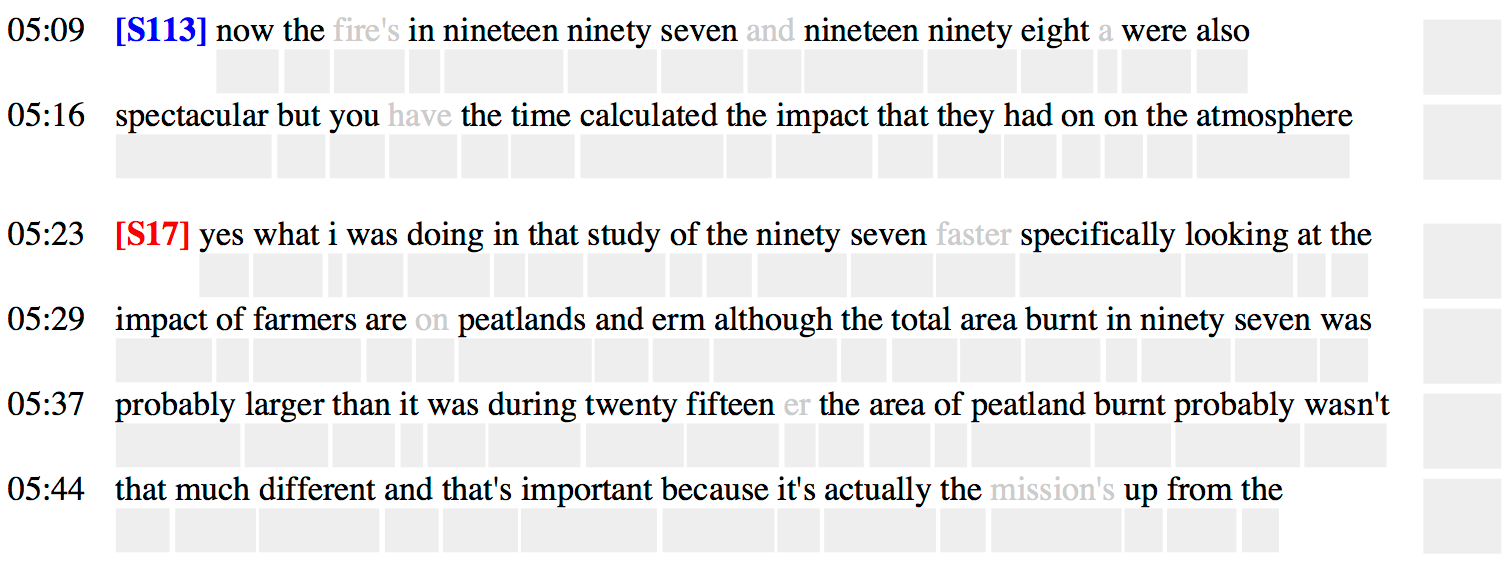
\includegraphics[width=\columnwidth]{figs/paper-prototype-design}
  \caption{Design of the paper prototype}
  \label{fig:paper-prototype-design}
\end{figure}

The transcript was generated using an automated speech-to-text system, which contained ocassional errors. We chose to
use this rather than a perfect transcript as we wanted to use automated transcription for the final system, and
removing the errors may affect user behaviour.

% Limitations of Anoto system, used normal pen for prototype
The Anoto Live Forms platform, which we used to create our system, works by dividing the page into rectangular active
zones.  When a digital pen draws inside one of these zones, that data can then be captured digitally and processed.
Traditionally this is used to detect when someone has ticked a box on a form, or to extract an image of a signature
drawn inside of a box.  To capture edit annotations that linked to the text of the transcript, we designed our layout
to use rectangular active zones that aligned with the location of each word.

% Edit commands: selector beneath word (double-spaced) and at end of line, removal by crossing word
From what we had witnessed from previous experiments, the most common annotations producers used were underline,
strikethrough and drawing a line down the side of the page.  To capture strikethrough, we drew an invisible active zone
on top of each word, so that when a line is drawn through the word, the zone is triggered. For underline, we draw a
shaded active zone directly below each word, so that drawing a line underneath a word triggers the zone. The transcript
was printed double-spaced to leave enough room for these boxes. Finally, we draw a shaded active zone at the end of
each line. Drawing a line through this zone would select the whole line.

% Additional features: paragraphs and speaker ID with gender, timestamp at start of line, confidence shading
The speech-to-text system we used provided additional information with the transcript.  Each word came with a timestamp
and a confidence rating. We wrote the timestamp at the beginning of each line in \textit{MM:SS} format, and used
confidence shading to grey-out lower confidence words.  The speech-to-text system also used speaker diarization
techniques to segment the transcript by speaker. This provided a speaker label and estimated gender for each segment.
We used paragraphs to segment the transcript, and wrote the speaker label at the start of each paragraph. We used blue
colouring for male speakers, and red for female speakers.

\subsection{Evaluation method}

%TODO Explain interview protocol and analysis

%TODO Why are participants asked to adopt three different strategies?

%TODO Explain design decisions, e.g. double-spacing, confidence shading

To evaluate our paper prototype, we ran a short experiment in which radio producers used our inactive prototype to
annotate real transcripts as if they were editing them.  We asked them to edit the transcripts in different ways, and
interviewed them afterward to compare the various approached. Producers are very busy, so to gain enough participants
in the time we had available, we designed the experiment so it could be completed within an hour.

We recruited five producers by using the contacts that we made from previous experiments. Two of the participants
worked in current affairs, two in science and one in documentaries.  The participants had between 7 and 13 years
experience working as a radio producer.

For the transcript, we asked each participant to provide us with a recent interview they had made, which we ran through
our speech-to-text system. We used this automated transcript for each participant's experiment so that they were
working with authentic speech, and a transcript that would be the same as that from a working system.

To help explore our questions about annotation and editing gestures, we directed participants to employ three different
strategies when using the prototype. This forced them to experience different ways of interacting with the prototype,
which they could later reflect on and compare. We instructed them to follow these directions for the first three
pages of their transcript: 

\begin{itemize}
  \item \textit{Page 1}: Undirected\\Edit the speech by annotating the transcript as you would normally.
  \item \textit{Page 2}: Underline only\\Edit the speech only by underlining words that you want to keep.
  \item \textit{Page 3}: Strikethrough only\\Edit the speech only by putting a line through words you don't want to keep.
\end{itemize}

The `undirected' strategy allowed us to see what gestures producers currently use, or want to use, without being
influenced by the design of the prototype or constrained by its limitations. We included the underline and
strikethrough strategies as we believed these to be the two most commons approaches, and we wanted the participants to
compare them directly.

We were also interested in learning about additional features and their value. To get feedback on the value of speaker
diarization, we produced two versions of each participant's transcript -- one with speaker diarization and one without.
The speaker information was used to segment the transcript into paragraphs, and the start of each paragraph was
labelled with the speaker identifier in square brackets (e.g.  \texttt{{[}S1{]}}).  For \textit{Page 4}, each
participant was presented with a transcript that included speaker diarization, and asked to edit the speech by
annotating the transcript any way they wished.

Timestamps, line selection and confidence shading were included with all of the prototypes. For these features, we
chose not to produce versions with/without as participants should be able to judge their value without having to see
them removed. Producing different versions for each would also unduly lengthen the experiment.

At the end of the test, we conducted a semi-structured interview with each participant. The following questions were
asked, but we also let the participants talk about whatever else they wanted to.

{\singlespacing
\begin{itemize}
  \item How do you normally use a pen to edit the transcript?
  \item Do you prefer to select parts you want to keep, or remove parts you don't want to keep?
  \item Which features of the prototype did you find useful?
  \item Were there any features missing that you would want added?
\end{itemize}
}

The experimenter wrote down the participants responses from the interview. These were then categorised into natural
gestures, edit gestures and additional features. We counted the frequency of each response within the categories to
see how popular the different approaches and features were. The participant's annotated transcripts were also
collected.

\subsection{Results}
The reaction to the system was overwhelmingly positive. All of the participants could immediately see the value of such
a system and most remarked that it would save them significant amounts of time and \textit{``revolutionise''} their
production workflow.

\subsubsection{Natural gestures}

The participants started the experiment by editing the transcript using any gestures they wanted.
Table~\ref{tab:natural-gestures} lists the gestures that were used, and by which participants.

\begin{table}[ht]
  \centering
  \begin{tabular}{|l|c|c|c|c|c|c|}
    \hline
                            & P1        & P2        & P3        & P4        & P5        & Count \\
    \hline
    Underline               & $\bullet$ & $\bullet$ & $\bullet$ & $\bullet$ &           & 4 \\
    \hline
    Strikethrough           & $\bullet$ & $\bullet$ &           & $\bullet$ & $\bullet$ & 4 \\
    \hline
    Line down side          & $\bullet$ & $\bullet$ & $\bullet$ &           & $\bullet$ & 4 \\
    \hline
    Comments                & $\bullet$ & $\bullet$ &           &           & $\bullet$ & 3 \\
    \hline
    Correction              & $\bullet$ &           &           &           & $\bullet$ & 2 \\
    \hline
    In/out marks            & $\bullet$ &           &           & $\bullet$ &           & 2 \\
    \hline
    Scribble-out mistake    &           & $\bullet$ & $\bullet$ &           &           & 2 \\
    \hline
    Lasso                   &           &           &           &           & $\bullet$ & 1 \\
    \hline
    Line through paragraph  &           &           &           &           & $\bullet$ & 1 \\
    \hline
  \end{tabular}
  \caption{Natural gestures used by each participant to edit their transcripts}
  \label{tab:natural-gestures}
\end{table}

\begin{figure}[h]
  \centering
  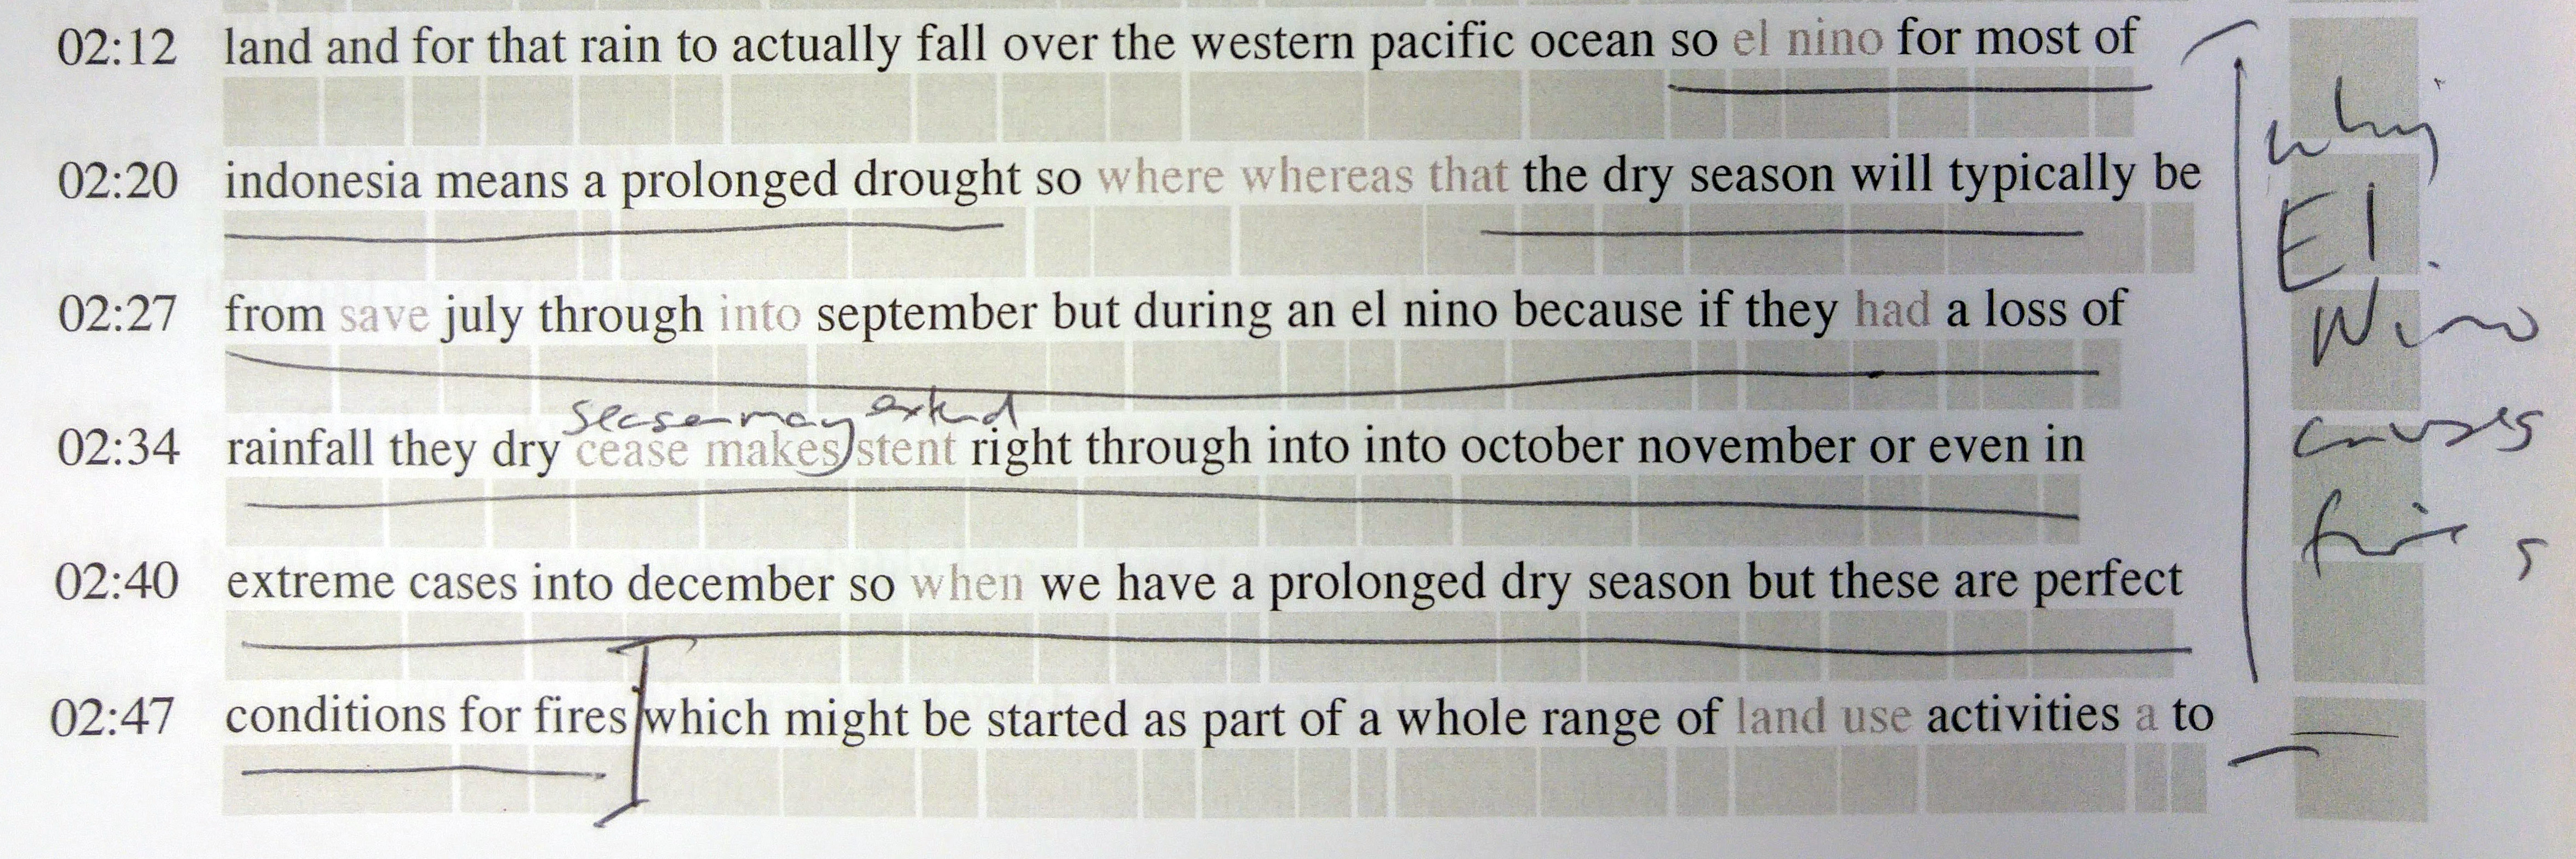
\includegraphics[width=\columnwidth]{figs/mockup-cropped}
  \caption{Paper prototype with natural annotations, including
    underlining, line down the side with notes, word corrections, and a
    vertical line to indicate the end of an edit.}
  \label{fig:natural}
\end{figure}

Four different gestures were used to select content -- underline, line down side, in/out marks and lasso.  Underline
was used by all participants but one, who was mainly interested in deleted unwanted content.  Drawing a line down the
side was used by three participants, as it is quicker and more efficient than underlining for selecting large chunks of
material.  Some participants combined both by using underline to be more precise about the start and end of their
selection.  One of the participants made a mistake when underlining, so scribbled out the underline to undo it.

`In/out marks' refers to drawing short vertical or diagonal lines before and after the words of a selection. These
indicate the in- and out-points for edits. One participant drew an analogy between these marks and the splicing of
magnetic tape, which was how radio programmes were edited before the digital age. `Lasso' refers to selecting a number
of words by drawing a line around them.

Two gestures were used to delete content -- strikethrough and drawing a line through a paragraph. These parallel the
underline and line down side gestures that are used for selection, but instead involve drawing a line through the words
themselves.
%TODO Expand

Finally, two participants corrected mistakes in the transcript by writing the correction over/above the
word, or to the side of the page.
%TODO Expand

Each participant used a different mixture of annotation techniques.
%TODO Expand

\subsubsection{Edit gestures}\label{sec:paper-proto-edit-gestures}
We asked each participant whether they preferred selecting or deleting words for editing the transcript.  P1, P3 and P4
reported that they preferred selecting, P1 commented that it \textit{``felt more natural''} to them and P4 said
deleting felt \textit{``counter-intuitive''}.

P2 and P5 reported that they preferred deleting words. P2 commented that \textit{``the challenge is to nibble away''}
and it was \textit{``the way my brain works''}. P5 said they prefer to \textit{``get stuff out of the way''}.

All of the participants were certain about which they preferred, but there was no overall consensus. Additionally, we
can see in Table~\ref{tab:natural-gestures} that all participants used a mixture of select and delete gestures during
the undirected annotation.

\subsubsection{Additional features}

% speaker diarization
Four of the five participants said that they found the paragraphs and speaker information useful. Typically, interviews
are recorded with a presenter and contributor, and the participants said they found it valuable to know when the
presenter is asking a question. Three of the participants said that they were able to find the questions much more
easily with this feature enabled. However, P2 said they found the speaker diarization to be \textit{``distracting''},
particularly when it was inaccurate.

% timestamps/confidence shading
All participants found the timestamps and confidence shading features useful, but P2 said that the timestamps are
\textit{``not needed on every line''} and P5 suggested that one timestamp per page would be sufficient. All of the
participants liked being able to select whole lines at a time. P5, who prefers to remove words, asked whether a similar
function could be available to delete content.

\subsubsection{Missing features}

During our testing, some participants suggested adding features that were not included, or used the prototype in a
way it was not designed.
% highlighting
P3, P4 and P5 remarked that they often highlight important bits of transcripts, usually with asterisks or stars.
P1 and P3 also suggested that the underline gesture could be extended so that underlining words twice marks them as
being more important.

% labelling, margins
Three participants made notes on the side of the page to label their content or to make a note for themselves. Due to
the limited space, the notes were often scrawled sideways in small writing. If the prototype was active, writing notes
on the transcript itself would likely have triggered the active zones located on and below each word. This would cause
the user to inadvertantly create edits to the audio. P3 suggested that it may be worth adding a margin. Providing an
inactive margin would give users a `safe space' to make freehand notes without editing the audio.

% correction
Two participants corrected words in the transcript by writing over or above the incorrect word. As the transcript was
double-spaced, there was just enough room between lines to write the correct word in small writing.
% listening/playback
P3, P4 and P5 expressed a desire to listen to the audio while reading/editing it, which echoes the importance of
listening noted in Chapter~\ref{chp:screen}.

%- Useful to know where presenter is asking question

%Diarization
%- Neal found it easier
  %- Shows where the questions are
%- Phil found it distracting
%- Wes found it absolutely useful
%- Marnie 'made it much easier', liked having paragraphs (usually one point per
%paragraph)


%Timestamps
%needed every couple of minutes

%Use L/R channels for presenter/contributor
%- Phil and Wes
%- Sometimes multiple on R channel (about one in eight interviews)

%Prefer landscape to portrait (landscape is `irritating' and doesn't match
%what's on screen)

%Whole line
%- Would like to delete line at a time

%Note-taking
%- One doesn't take many notes

%Correction
%- One corrects then selects edits
%- Wes would like option

%Highlighting
%- Asterix/star to mark important bits (Phil, Neal)
%- Underline twice (Neal, Marnie liked idea)
%- Wes sometimes double-stars

%Delete vs select (2 vs 3)
%- Phil likes to `get stuff out of the way'
  %- Words that aren't marked should be kept by default
  %- Underline should undo delete
%- Neal prefers selecting over deleting
  %- Delete should undo select, if underlined too far
%- Wes prefers selecting - deleting is `counter-intuitive'
  %- Would like delete to override select, but would like options for opposite
%- Marnie found it trickier to delete than select, selection is more natural
  %- worried about deleting something good
%- Alex feels delete is more natural, 'way may brain works, 'challenge is to
%nibble away', thinks delete should be active, select should override delete

%Margin
%- Phil wouldn't need a margin
%- Neal would like one

%Export
%- gaps should be put between edits (real-time?)

%Transcript
%- Phil and Neal no problems
%- Wes had problems (strong Scottish accent) made it unusable

%Observation
%- Neal
  %- underlined as he read (unprompted), scribbled out when mistake made
  %- found it more difficult to only delete
%- Wes
  %- vertical lines for in/out points

%Other
  %- Neal would like to press and hear word (on laptop?)
    %- Wes: Don't know what sounds good
  %- Wes works in a team of 3/4. They use Box to collaborate
  %P4 reported that they usually work in teams of 3 or 4 people. They use Google Docs to collaborate on a central
  %programme script, so they can all edit the document simultaneously.

\subsection{Discussion}

In this section, we set out to answer three questions about the gestures producers use to edit printed transcripts, and
which features we should include in our paper-based audio editing interface. We did this by evaluating a paper
prototype of our interface on five radio producers using real content.

  %\item What gestures are currently used by radio producers to annotate transcripts?
  %\item Do producers prefer to select content they want to keep, remove content they don't want, or a mixture of the
    %two?
  %\item Which additional features (e.g. timestamps, speaker labelling, confidence shading) should be included in the
    %layout?

We observed that the participants used a variety of gestures to select and delete content, with underline,
strikethrough and a line down the side being the most common.  This confirms our assumptions about these being the most
popular annotations, which drove the design of our prototype.  The other gestures included in/out marks and lasso for
selection, and drawing a line through a paragraph for deletion.  In \citet{Weibel2008}, strikethrough was also used for
delete, but something similar to in/out marks was used for annotating a specific region.

There were mixed but strong opinions on whether it was better to select good content or remove bad content.  Most
participants used a mixture of both approaches when undirected. Given the lack of consensus, it would be best to give
producers the option to do both, but this raises the issue of what should happen when a word is both selected and
deleted.  If one overrides the other, then it could function as an undo mechanism. The more conservative approach would
be for selection to override deletion, so that speech can always be recovered. However the system does not delete any
audio, so this is not a risk.

Selection and deletion could be used together at different scales, where one is used to select/delete large chunks,
then the other is used to refine the choise by selecting/deleting smaller words or chunks within the larger ones. In
our results, we saw that selecting large chunks is more popular than deleting large chunks. Also, there is likely to be
more interest in removing individual words, such as for `de-umming', than there is for selecting individual words. For
this style of use, it may be better for delete to override select.

When underline is used to select content, it implies that everything else should be discarded except for the underlined
parts. Alternatively, underline could be used to highlight parts of interest. In a later stage, the user could then
choose to either keep everything except the deleted words, or to keep only the highlighted words minus the deleted
words. This would give greater flexibility to different modes of use, like we saw in
Section~\ref{sec:paper-proto-edit-gestures}.

Most participants valued the additional features we tested -- speaker diarization, timestamps and confidence shading,
but reported that timestamps on every line are unnecessarily frequent. During our testing, we also identified missing
functionality for labelling, correction, highlighting and playback.

% Missing features
Handwritten text was also used to make
corrections to the transcript, and to label parts of the transcript.

% labelling
Three participants made notes on the side of the page to label their content or to make a note for themselves. Two of
the participants remarked that there was no free space in which to make notes, and suggested that it may be worth
adding a margin. Writing notes on the transcript itself would trigger the active zones that are on and below each word.
Providing an inactive margin would allow users to make freehand notes without inadvertantly making edits to the speech.

% correction
Two participants corrected words in the transcript by writing over or above the incorrect word. 
Potentially users could write the replacement word in an active zone, but...

% highlighting
Most participants remarked that they normally mark important bits of the transcript, often with asterisks or
stars. Underlining twice could also introduce a two-tier selection system.
Possibly the side boxes could be used to rate or star a selection.

% playback
Some participants expressed a desire to listen to the media from the paper interface, and this functionality has been
shown to be useful in previous work. %TODO Reference
An external device, such as a phone, computer or portable media player could be used to replay the audio while using
the paper interface.

Users could start playback by pressing a word with the digital pen. This could be
achieved either by wirelessly linking the digital pen to a computer that plays the content, or by storing the audio on
the pen itself similarly to the LiveScribe Sound
Stickers\footnote{\url{http://store.livescribe.com/sound-stickers-1-1.html}}.

% natural annotation:
% underline, strike and line down side most used, reinforced design decision
% comments and correction were popular, no space to write them
% in/out marks, lasso also used for selection, line through paragraph used for deletion, but to lesser extent

% edit gestures:
% no consensus on best approach, both used when naturally annotating, so both should be available
% what to do when using both? underline override strike or vice-versa?

% additional features:
% speaker diarization - yes
% timestamps - yes, but less frequently
% confidence shading - yes


%Our system performs the same function as these systems, but uses a paper
%interface rather than a screen-based one.
%Our system
%similarly interprets the paper annotations and applies them to the media
%content.
%Our system does not yet have the ability to replay content from the
%paper interface, but this is a feature that could later be included.
%Our system is based on printed transcripts rather than video frames on
%a tablet, but approaches the same problems from a different angle.
%These systems do not provide the user with any pre-written notes.
%Our system uses speech-to-text to generate a transcript, which the user can
%then annotate further.
The participants used a variety of techniques to annotate the transcripts, but underline, strikethrough and lines down
the side were common. There were strong but mixed opinions on whether selection of desired material, or removal of
unwanted material, was the best approach to use for editing, so we decided to make both options available.

%TODO What happens when underline and strike same word?

\section{System design}\label{sec:paper-design}

%TODO Why are some desired features not included, e.g. vertical lines for in/out, lasso

%TODO How are the results of the edit presented back to the user?

%TODO Underline/strikethrough interaction


Using the feedback gathered from our requirements gathering, we designed and implemented a working prototype of the
paper-based semantic speech editing system. To build our system, we collaborated with Anoto to use their Live Forms
platform. We integrated the paper interface with an updated version of our screen-based semantic speech editor, so that
it could support audio input and output.  In this secton, we will explain the design of the paper-based interface and
its functionality, and the updates we made to the screen-based interface.

\subsection{Paper interface}

We used the results of our paper prototyping experiment to inform the design of the interface for our paper-based
semantic speech editor. We will explain the design choices that we made, describe the layout and functions of the final
system, and show how we added audio input and output by integrating it with our screen-based interface.

\subsubsection{Design decisions}

We chose to use three methods for selecting and deleting material - underline, strikethrough and line down the side.
We did not include in/out marks, lasso or drawing a line through a paragraph as these were not as popular, and would
have been much harder to detect using the Anoto Live Forms system.

We included speaker diarization and confidence shading, as the majority of participants in the paper prototype found
these valuable. We also chose to keep timestamps, but opted to reduce the frequency to one timestamp per paragraph,
rather than on every line. We expected this to provide a sufficiently narrow search reason without occupying more space
than necessary.

We added a margin to allow users to write freehand notes without the risk of accidentally editing the audio. We did
this by drawing a rectangular box on the right side to indicate where the user could safely write.
We set the margin to be approximately 25\% of the width of the page, based on informal feedback from producers.
For the margin, we decided to allow users to draw freehand in the margin, rather than attempt to structure and capture
these annotation. We did this because of the variety of annotations and techniques producers use for annotations.

In the paper prototyping experiment, we saw that some participants wrote corrections on or above wrongly transcribed
words. However, we chose not to include any correction functionality, partly due to the limitations of the Live Forms
system, and partly to keep the interface simple. The active zones on or below each word could be used to write
corrections, but this would prevent underline or strikethrough gestures being used. The correct word would have to be
written within these active zones, which are quite small. Corrections often span more than one word, which would be
difficult to detect.

We did not include any linked playback features as this would require a live wireless link between the pen and a
playback device. The system we used to build our system only operated in batch mode, where the pen must be
connected to a dock to upload the recorded gestures. Although this prevented the user from navigating the audio using
the pen, they could of course replay the audio on a separate device and use the timestamps to navigate to the correct
location.

\subsubsection{System description}

This section describes the final design we used for the paper interface for our semantic speech editing system.
Figures~\ref{fig:paper-interface-diagram} and \ref{fig:paper-interface-example} on page
\pageref{fig:paper-interface-diagram} show the final design of the interface.

\begin{figure}[p]
  \centering
  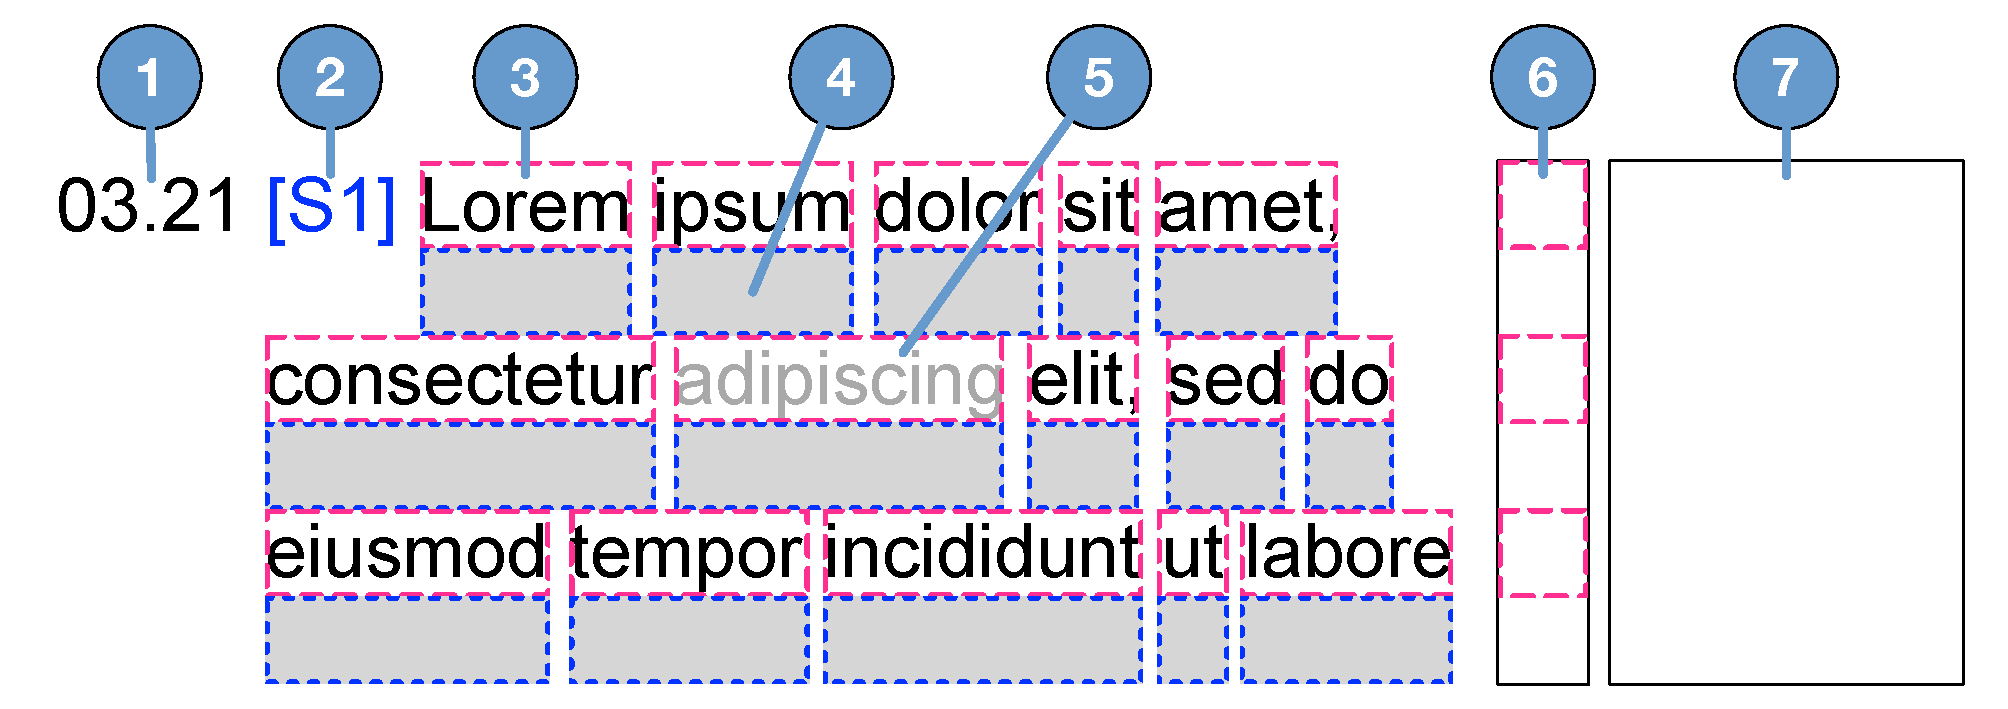
\includegraphics[width=\columnwidth]{figs/paper-interface-diagram.pdf}
  \caption{Diagram of the paper interface layout with timestamps at beginning of each paragraph (1), speaker
  diarization (2), word selection (3), word deletion (4), confidence shading (5), line selection (6) and a margin for
  freehand notes (7). Dotted lines indicate hidden active zones for selection (pink) and deletion (blue).}
  \label{fig:paper-interface-diagram}
\end{figure}

\begin{figure}[p]
  \centering
  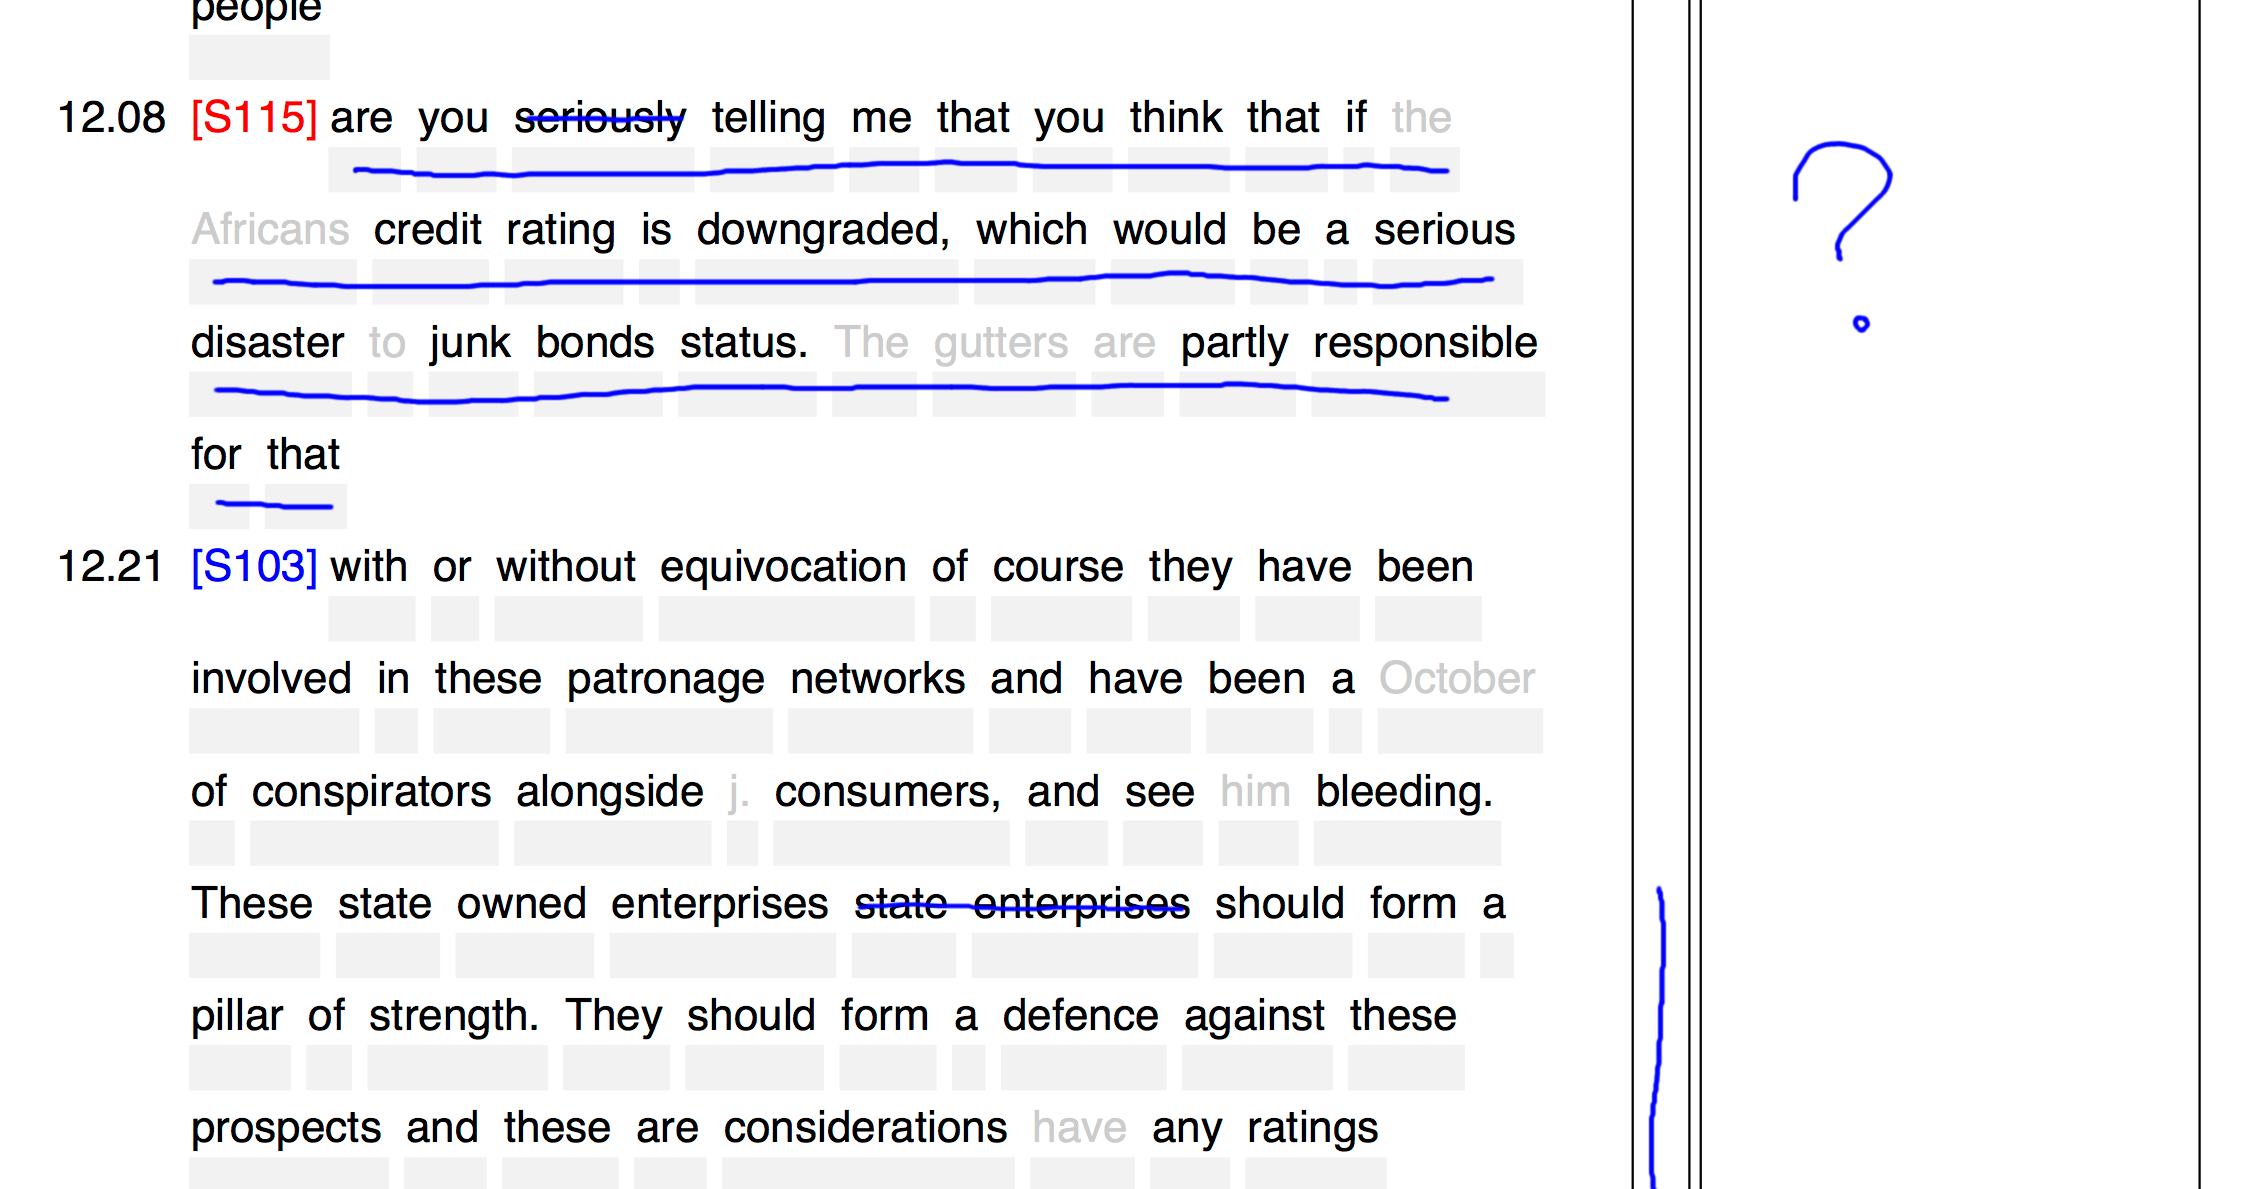
\includegraphics[width=\columnwidth]{figs/paper-interface-example-annotations.png}
  \caption{Example of the paper interface system, with freehand annotations that demonstrate its use.}
  \label{fig:paper-interface-example}
\end{figure}

For each word in the transcript, two rectangular active zones are defined on the page -- one on the word itself and
another in the space directly below the word.  Any marks made on or below the word label that word as `deleted' and
`selected', respectively.  This allows the user to use a digital pen to delete words using a strikethrough, or to
select words by underlining.  The zone below is lightly shaded so that the user can see where the boundary lies between
the two regions.

For selection by drawing a line down the side, we opted to draw a long thin rectangle from the top to the bottom of the
page to the right of the transcript, rather than draw individual square boxes at the end of each line. We did this to
save some space, and to align with how the participants used the paper prototype.

The paper must be annotated using an Anoto Live Pen 2. This records the gestures made by the users digitally on the
pen.

To include audio editing functionality with the pen system, we integrated it with a screen-based interface. A diagram
of this integration is shown in Figure~\ref{fig:paper-screen-integration}. The screen
was used for asset management, including uploading new content and printing the transcript, and for viewing/changing
the edits made using the pen, and exporting the resulting audio or edit decision list.

When the pen is connected to its USB dock, the gestures are automatically uploaded to some Anoto software running
on the local computer, which processes the information from the pen. This is then sent to our server, which creates an
edited version of the transcript. This can then be accessed through the screen interface.

In addition to creating an edited version of the transcript, a PDF document of the transcript with the user's
annotations is created. This PDF can be viewed through the screen-based interface, so that they can refer to any notes
they made in the margins.

The user can export the audio from the edited transcript using the screen interface. Two types of export format are
supported. The user can download an EDL of the edits for either the SADiE or StarTrack audio editing systems.
Alternatively, they can download an edited version of the audio as a WAV file.

\begin{figure}[ht]
  \centering
  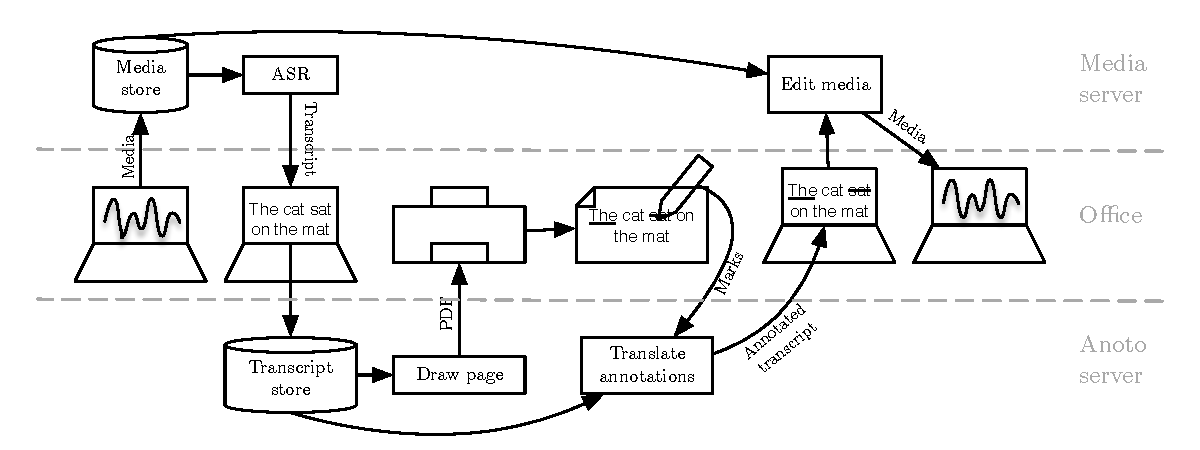
\includegraphics[width=0.5\columnwidth]{figs/uist-sys-diagram}
  \caption{Integration between the paper and screen interfaces, flowing from top to bottom.}
  \label{fig:paper-screen-integration}
\end{figure}

\subsection{Screen interface}
We updated the screen-based interface used in Chapter 5 to integrate the changes suggested by our findings. This gives
us something which we can compare the paper-based interface with.
The previous screen-based system is shown in Figure~\ref{fig:interface} on page \pageref{fig:interface}, and the
updated interface is shown in Figure~\ref{fig:dialogger-interface} on page \pageref{fig:dialogger-interface}.
The two major differences are that underline and strikethrough are used instead on drag-and-drop, and that only one
recording can be edited at any one time.

\subsubsection{Design decisions}

We replaced drag-and-drop with an underline/strikethrough method for three reasons.
Firstly, we found that there was not enough room to handle large clips, which was what most users were interested in.
Secondly, we found that users mostly used the tools for rough editing, so weren't as interested in mixing different
recordings together. This meant that we could concentrate on one file at a time.
Finally, we wanted the edit scheme to match our paper-based interface, as this would allow us to compare the two
modalities side-by-side.

There were many other smaller changes we made to the interface. We added double-speed playback to allow users to listen
faster than real-time, as requested by participant in our previous experiment. Previously, users could only make a
single edit per project. For the updated version, we allowed users to make multiple different edits of the same
recording by separating the original 'media' from the modified 'edits'. We also added a Save As button so that edits
could be branched.

We adjusted the speaker diarization display using a line down the side of each paragraph, coloured by gender and with a
label to the left to distinguish between speakers. We included confidence shading, but opted to use a dotted red
underline to indicate low confidence in order to match the style of word processors, and also to make it clearer.

\subsubsection{System description}

Users can login using their normal BBC account. They are then presented with the edit screen, which
has hidden sidebars on the left and right. Media that is uploaded is stored on the left-hand side, and any edits are
stored on the right-hand side. Edits can be exported either as an EDL or as an edited audio file. Users can only edit
one recording at a time, and multiple recordings must be mixed together at a later stage. Speakers are shown by a line
on the left of each paragraph, and any words with a low confidence are underlined with a dotted red line.

\begin{figure}[p]
  \centering
  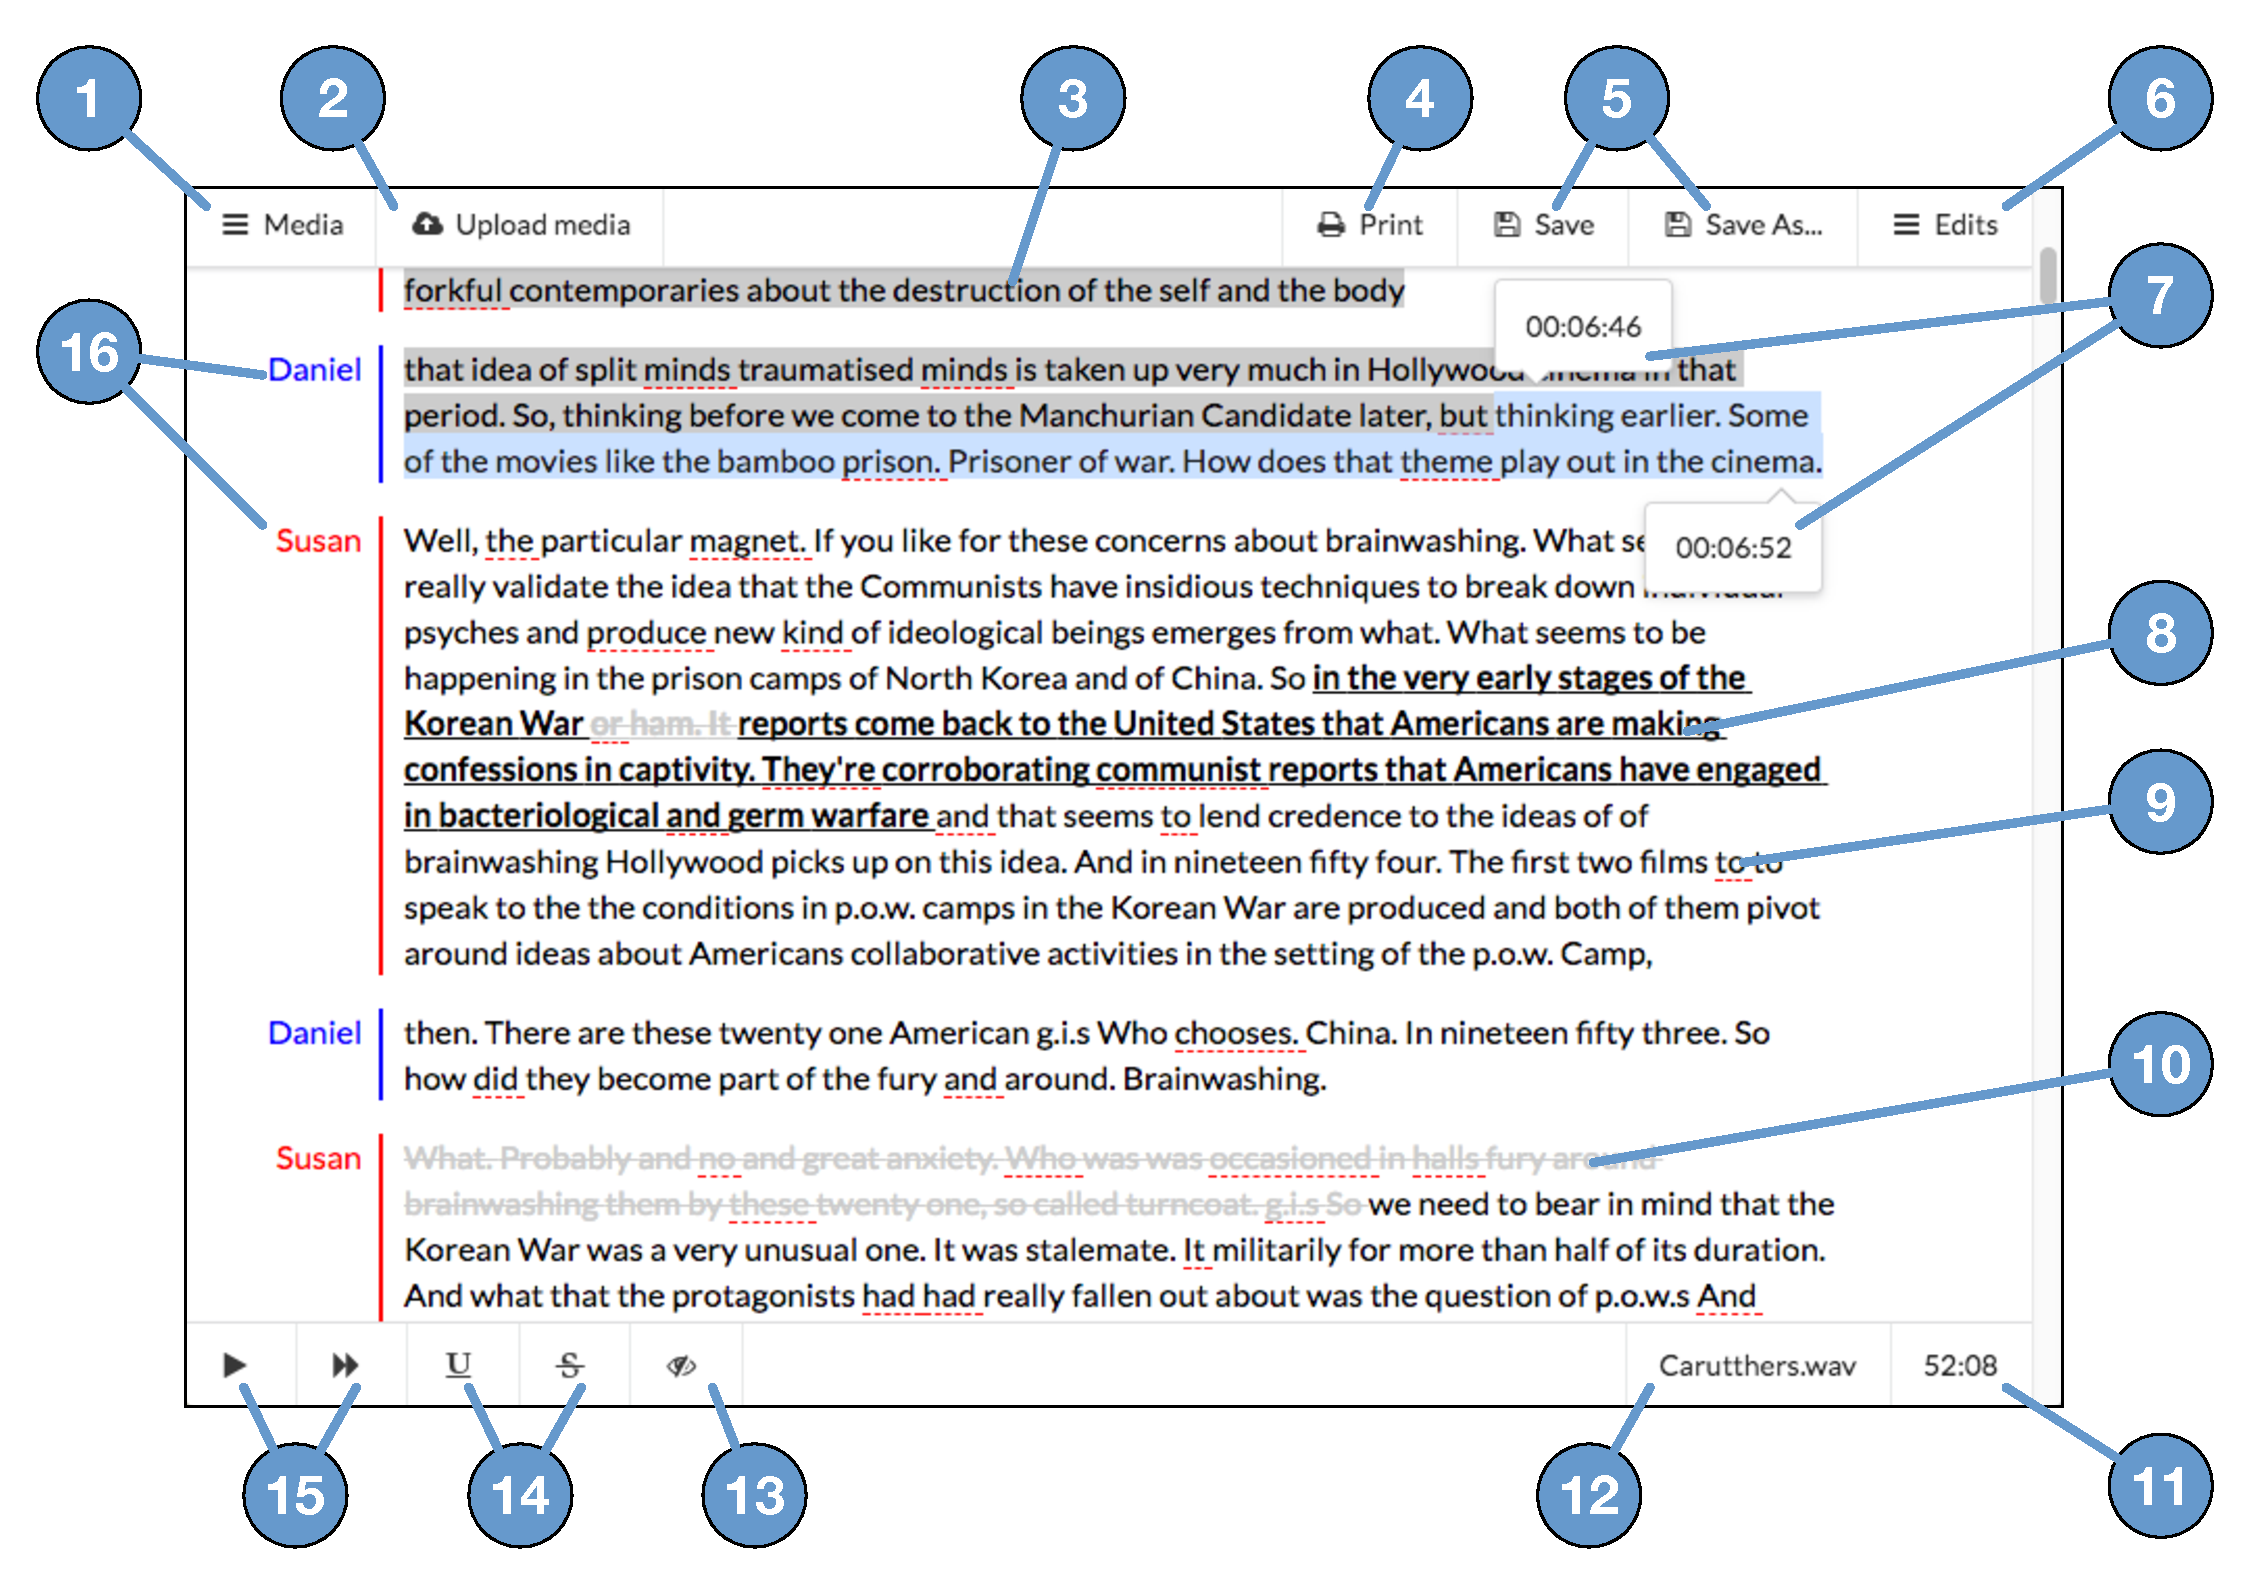
\includegraphics[width=\columnwidth]{figs/discourse-interface-labelled.pdf}
  \caption{Layout of the screen interface, which features 
    media storage (1),
    media upload (2),
    highlight of the current playback position (3),
    printing the transcript (4),
    saving edits and corrections to transcript (5),
    edit storage and export (6),
    displaying timestamps of the current selection (7),
    underlining words (8),
    confidence shading (9),
    strikethrough of words (10),
    display of edited audio duration (11),
    name of current asset (12),
    show/hide strikethrough (13),
    underline/strike buttons (14),
    playback buttons (15)
  and speaker diarization (16)}
  \label{fig:dialogger-interface}
\end{figure}

\begin{figure}[p]
  \centering
  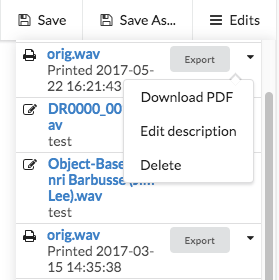
\includegraphics[width=0.4\columnwidth]{figs/discourse-download-pdf.png}
  \caption{Close-up of the edits sidebar showing the button to export audio, and the option to download a PDF.}
  \label{fig:download-pdf}
\end{figure}

\section{Evaluation methodology}\label{sec:method}

To compare the paper and screen interfaces, we designed and conducted a user study.
The objective of our study was to 

\subsection{Design and procedure}
We ran a within-subjects user study in which we tested three different conditions: the paper interface, the screen
interface and a printed transcript. The printed transcript acted as a control, and was inactive in the sense that it
did not make use of the Anoto dot pattern technology.  The transcripts for all three conditions were generated by the
same speech-to-text system. In this study, we did not want to test the impact of the transcript itself, but rather
impact of the interface that is used to interact with the transcript.

We recruited professional radio producers exclusively from BBC Radio so that we could take advantage of the access that
was available to us. We recruited participants by sending an invitation by email to the current affairs, science and
documentaries teams in BBC Radio.  Through this, we recruited eight participants who had between 8 and 28 years
experience of professional radio production, with a mean average of 16 years experience.

We asked each participant to provide the audio recordings from three recent interviews they had made, so that the
content was genuine and fresh in their mind. We set a minimum duration of 20 minutes for each recording, as we found in
our previous study that there was no much advantage in using transcript-based editors for short recordings.

We divided our study into three stages, explained below:

\paragraph{Stage 1: Training}

Firstly, the participant was briefed on the study and asked to sign a consent form.  We then trained the
participant on the paper and screen interfaces using a test recording.  The experimenter explained all of the features
of the interfaces, and asked the participant to perform a sequence of actions based on a script. This allowed the
participant to use and experience all of the features for themselves. The participants were given the opportunity to
ask questions and play with each interface until they felt comfortable with how they worked and could be used.

\paragraph{Stage 2: Observation}

The second stage of the study was observing the participant edit three different recordings, each under one of the
three conditions.  The order of the conditions was counterbalanced to avoid carryover effects.  The tasks performed by
the participants overlapped with the work they needed to do already, which ensured that the tasks were genuine.  We
needed to use different recordings for each condition to ensure the tasks weren't just being repeated, but we asked the
participant to choose recordings from the same programme to ensure they were as similar as possible.

The observation took place at the participant's normal work environment, which in all cases was at their desk in an
open plan office. As the systems we built could be accessed using a web browser, the participant used their own
computer and desk. We considered recording the task using a video camera, but chose not to as we wanted to run the
study in the normal work environment. Due to the open-plan nature of the offices, this would have caused problems with
information security.

During the observation, the experimenter sat beside the participant and made written notes detailing what the
they were doing, and noting anything of interest. If the participant had any `down-time', the experimenter used this to
clarify anything they didn't understand. Items of interest included:

The specific items of interest at this stage include:
\begin{itemize}
\item Editing workflow
\item Tools used
\item Data generated
\item Usability challenges and problems
\item Navigation and edit actions
\item Time taken to complete tasks
\item Unexpected reactions
\item Unanticipated usage
\end{itemize}

During each task, the experimenter kept track of how long it took the participant to complete the task, excluding any
time not spent on the task at hand (e.g. phone calls, making tea). We also logged the length of each recording being
edited.  After each task was completed, the experimenter asked the participant to fill out a questionnairre to measure
the usefulness and usability of the interface using the Perceived Usefulness \citep{Davis1989} and Software Usability
Scale \citep{Brooke1996} metrics, respectively.  Photographs were taken of the paper annotation and work environment,
with the participant's permission.

{\singlespacing
\begin{itemize}
  \item Using this system in my job would enable me to accomplish tasks more quickly.
  \item Using this system would improve my job performance.
  \item Using this system in my job would increase my productivity.
  \item Using this system would enhance my effectiveness on the job.
  \item Using this system would make it easier to do my job.
\end{itemize}
}

{\singlespacing
\begin{itemize}
  \item I would find this system useful in my job.
  \item I think that I would like to use this system frequently.
  \item I found the system unnecessarily complex.
  \item I thought the system was easy to use.
  \item I think that I would need the support of a technical person to be able to use this system.
  \item I found the various functions in this system were well integrated.
  \item I thought there was too much inconsistency in this system.
  \item I would imagine that most people would learn to use this system very quickly.
  \item I found the system very cumbersome to use.
  \item I felt very confident using the system.
  \item I needed to learn a lot of things before I could get going with this system
\end{itemize}
}

After completing all of the tasks, we asked the participant to fill out a form to measure user preference. The form
simply asked

\textit{``Of the three systems you have just tried, which of them would you most prefer to continue
using?''}

and had a checkbox for each of the three interfaces.

\paragraph{Stage 3: Interview}

For the final stage of the study, the experimenter performed a semi-structured interview with the participant. This
gave the participant the opportunity to discuss each of the three conditions in detail and compare them directly. An
audio recording was made of the interview, which was used to perform in-depth analysis.

We asked the participant the following questions:

{\singlespacing
\begin{enumerate}
  \item Can you please describe your existing process for editing audio?
  \item What did you like or dislike about the paper-based system?
  \item What did you like or dislike about the screen-based system?
  \item What did you like or dislike about using normal paper?
  \item Overall, which of these systems would you prefer to continue using, and why?
\end{enumerate}
}

The first question was included to understand more about the participant's current approach, in case that affected
their preferences or usage of the systems.  The order of questions 2--4 were adjusted to match the order in which the
conditions were presented to the participant.  The final question gave the participant an opportunity to expand on the
decision they made at the end of Stage 2.

\subsection{Analysis}

We performed both qualitative and quantitative analysis on the data we collected during our study.

For the qualitative analysis, we transcribed all of the audio recorded during the interviews by using our screen-based
interface to run speech-to-text and then correcting the words manually. This process produced 23,000 words of
transcripts. Using grounded theory, the principal investigator then openly coded the transcripts using the RQDA
software package. This produced 116 different codes. The principal investigator used mind-mapping software to group
these codes into 17 categories, then grouped the categories into three high-level themes. RQDA was also used to extract
representative quotes from the interviews to illustrate the points made.

During the study, we collected data about task duration, system preference, usefulness and usability.
We plotted the task duration measurements against the duration of the audio being edited. For each condition, we drew
the linear regression to see how the edit time is affected by longer or shorter recordings, and to compare the the edit
time of the three conditions.
The questionnaire data measuring the usefulness and usability were separately converted into scores between 0 and 100.
This follows the procedure described in \citet{Davis1989} for usefulness, and \citet{Brooke1996} for usability.
For the system preference data, we simply reported the count of the participants' preference for each system.

\section{Study results}\label{sec:paper-results}

In this section, we will present the qualitative results that emerged from the interviews with the participants,
followed by the quantitative data that we also collected.  The codes that resulted from the analysis of the interview
transcripts are shown in Table~\ref{tab:paper-codes}. Three themes emerged from the coding process -- `editing',
`transcript' and `listening' -- and we will present them below individually. 

% P7 already used speech-to-text as part of his process, unusual

\begin{table}[h]
\centering
{\small
\begin{tabular}{|p{0.18\linewidth}|p{0.2\linewidth}|p{0.5\linewidth}|}
\hline
\multirow{5}{*}{Transcript}
 & Paper & Multiple windows/tabbing, Can't print on location, Quantity of paper (high), Takes time to print, Physicality, touch, Better, faster comprehension, Use of finger/pen to navigate, Bimodal reading/listening is better, Improves memory \\ \cline{2-3}
 & Accuracy & Use of memory affects threshold, Field recordings, Affects speed, Punctation (distracting), Good enough, Speaker diarization, Affects amount of listening, Accents, Noise, Affects edit resolution, Doesn't show umms/breaths \\ \cline{2-3}
 & Generation & Skipping/paraphrasing, Clerical job, Simultaneously making edit decisions in head, Takes too long, Third-party, overnight, Turnaround time, Question marks, Cumbersome/tedious \\ \cline{2-3}
 & Correction & Depends on length (don't need to for shorter), Not on paper, Fix repeat errors, For giving to other people, PasB transcript \\ \cline{2-3}
 & Technique & TV (thumbnails, expense), Search archive material, Compare and orientate other recordings from programme \\ \hline
\multirow{8}{*}{Editing}
 & Collaboration & Easier with digital representation (screen), Remotely, Compare notes with presenter, Timecodes or page/line numbers for reference, Side-by-side comparison, Google Docs, Share new material with presenter, With third-party institutions \\ \cline{2-3}
 & Annotation & Colours, Highlight, Summary (auto?), Star, Labelling/numbering (auto?), Freehand, Speaker names, Music information \\ \cline{2-3}
 & Location & Thinking space, Away from desk/screen, Downtime - plane/train/bus, Quieter, Concentration \\ \cline{2-3}
 & Export & Transcript and annotations in DAW, Move selections to different track, Spaces between exported clips \\ \cline{2-3}
 & Pen & Narrow margin, Could be lost/broken, No correction, Cost, Can't draw freehand, only strike/underline, Note digitisation, Poor ergonomics, Desired gestures, Simplicity/lack of functionality, Lack of undo (same as normal pen), Must be precise, Easier to edit without interrupting playback, Higher edit precision, Permanency increased decisiveness \\ \cline{2-3}
 & Technique & Re-ordering and mixing (cut/paste), Pull out good bits, Remove bad bits, Rough edit first, Check nothing's been missed, Taking too much at early stage, Simultaneous correct and edit, Top and tail, Paper edit only (no listen), Multiple iterations (re-print) \\ \cline{2-3}
 & Decisions & Must be made in real-time, Easier to decide with paper, Simultanous listening/editing easier on paper \\ \cline{2-3}
 & Interface & Familiarity, Learning curve, Auto-labelling?, Limited options (faster?), All in one place, Editing large chunks, Training/cheatsheet, One of many different systems \\ \hline
\multirow{4}{*}{Listening}
 & Speed & Discourse x2 playback hard to understand, Use memory to skip, Faster with transcript \\ \cline{2-3}
 & Navigation & Can use finger as cursor on paper, Jumping around (easier with DAW), Timestamps, Reading ahead, Space bar to start/stop \\ \cline{2-3}
 & Criteria & Intonation, Works on paper, not on audio, Transcript accuracy, Do clips work on their own/together?, Sound effects (e.g. thunder), Umms, Breaths, Does edit work?, Is transcript correct? \\ \cline{2-3}
 & Technique & Process/reinforce information, Fine editing, 'Listening is editing', Mental buffering during de-umming \\ \hline

\end{tabular}
}
\caption{Themes, categories and codes from the interviews.}
\label{tab:paper-codes}
\end{table}

\subsection{Editing}

\subsubsection{Edit technique}

% ITERATION

Participants reported that editing was an iterative process, not just a single stage. Many participants reported that
they did a rough edit first to either get rid of the worst bits that they definitely weren't going to use, or to pull
out the best bits that they definitely were going to use.

There did not seem to be a consensus on the best of these two options. Some were interested in a 'slash and burn',
whilst other wanted to pull out the best bits first.

The reason behind the iterative process was that there are a number of unknowns when the producer starts editing. They
do not know exactly what the narrative will be, as this can often change throughout each interview, and depend on what
is said in other interviews. They also do not know how long the material needs to be - they may need a lot of material
as there is not much good stuff in other interviews, or they may take way too much as the other interviews were better.

If they take too much, then they will have to reduce their selection down further at a later stage. If they don't take
enough, or take the wrong pieces, then they will have to go back to extend their selection or change it for a
difference piece.

As they put the programme together, they will also have to reduce the programme down to a specific time. Radio
programmes must be edit to fit an exact time slot, so towards the later stages of editing, the producer must reduce
their selections to a specific time.

Throughout the editing process, the participants were making edit decisions. Some were reported to be easier than
others, so most opted to perform a multi-stage edit, where the obvious edits are done first, and the less obvious ones
are done later. This then allows them to spend more time focussing on the most difficult edits.

One participant used the transcript to go back after their editing to ensure that nothing important was missed in the
material they had not used.

One participant suggested using different colours in the pen to indicate the multiple stages on an edit, so for
example, using red for the first pass, blue for the second etc.

P6 said they would have liked to perform multiple editing iterations using the pen interface, but were unable to using
the current design. They suggested that it may be possible to use different colour pens for each iteration, so that
they could be distinguished. For example, a red pen would show the edit gestures for the first iteration, blue for the
second etc. Implementing this would require an easy way for swapping the ink in the pen, which is currently not
possible without using tools.

% LABELLING

In addition to selecting/removing content, the participants were also interested in organising their content. Several
reported an interest in assigning labels to segments while they edited, and another wanted to name each of the clips
they selected from the material.

% RE-ORDERING

After rough editing their material, the participants wanted a method to order their selections into a rough narrative
to see how it would work. This is analagous to cut-and-paste in word processing, where items are moved around. The idea
is to help the producer piece together an interesting narrative from the pieces they have selected from their
interviews.

\subsubsection{Edit decisions}

% READING AHEAD/BEHIND

Making edit decisions is easier to do when the interview is fresh in memory, and most likely requires less
re-listening. Therefore it is benefitial to start the editing process as soon after recording the audio as possible.

Having a transcript was reported to aid the edit decision making process in several ways. It allowed participants to
read ahead of their current listening position to see whether the material coming up was going to be interesting or
relevant enough to bother listening to. This can potentially save on the listening time needed for this process.

P5 said the transcript helped them keep track of which interview they were currently editing. For a single programme,
there will be multiple interviews recorded which has the potential to be confusing as to which interview the
participant is currently editing.

Many participants talked about their motivation for navigating around the audio recordings while listening. P2 and P5
talked about how they would hear something that would cause them to use the transcript to read what had happened
previously to judge the relevance of what they had just heard.

The most common reason cited by participants was to use the transcript to read ahead while listening. P2, P4, P5 and P7
talked about how what they heard would occassionally push them to read further down the page to see whether it was
worth continuing to listen, or whether they should not bother. This was used as a time saving tool, which would not be
possible in an audio-only editing workflow.

% REAL-TIME EDITING

Having the transcript printed out on to paper was reported to make the edit decision process easier.

P4 reported that the limitations of the pen-based interface made the decision-making process faster. Without the
distractions of additional features such as correcting the transcript or navigating the audio, they were better able to
concentrate on deciding whether to keep or lose the piece of audio under consideration. P4 and P8 said that this
allowed them to edit the audio in real-time, as the audio played without pausing. This was said to be very unusual
[quote].

However P5 reported that this method of editing in real-time took some adjusting. They also thought that they were
selecting more content than usual so that they didn't miss anything.

% DECIDING ON PAPER

It is already known that reading from paper rather than a screen improved comprehension, but P8 reported that they
found it easier to made their editorial decisions on paper compared to the screen. [quote] It's possible that the
improved comprehension of physical paper may decrease the load of the task, allowing them to make decisions faster.

P7 felt that the pen system gave a different dynamic to the screen. They viewed the pen system as a way to make fast
decisions on whether to keep or remove something.

\subsubsection{Interface}

% ALL IN ONE

P3 and P6 said they enjoyed that the screen had all of the features available in the same place. The playback of the
audio was integrated into the interface, and they could correct and annotate the text, then export it without having to
move between systems.

% LEARNING CURVE

There were mixed reports on the learning curve of using the screen. P3 thought that it was only a small step from word
processing, but P7 and P8 thought there was a larger learning curve

The learning curve for both interfaces was considered to be pretty short. P3 thought that the word processing style
interface of the screen made it very familiar, but P8 found it tricky to get used to and P7 thought it could benefit
from having some instructions.

% COMPARISON

Several participants felt as though the existing workflow was the most comfortable or easiest of the three conditions
we tested. P7 said that having a printed transcript was useful as an aide memoire.

P7 reported that editing using the pen would be faster than the screen if the interview was done recently, as they
would not need to refer to the audio. It is possible that the pen is quicker in situations where the audio does not
have to be referred to as often.

P2 and P7 said that they thought the screen and pen interfaces both had strengths in different areas, so there was a
benefit in having both options available. The screen may be better for more intensive editing where producers may not
be sure what they want from a recording. The pen system may be better for quickly selecting and removing content when
it is known what is needed.

This may be due to the ease of navigating the audio in the screen interface, which is not present in the pen. This is
because a separate device must be used for playback, and this is not linked to the words. This makes it more difficult
to navigate non-linearly, which could be the reason for it being preferred for editing straight-through. Another reason
could be because the pen interface has fewer features, so is seen as a more lightweight option against the feature-rich
screen interface.

Some participants preferred the normal printer paper transcript to either of the semantic editing interfaces, as it was
more familiar to them. It allowed them to use their existing tools, which they used regularly, and therefore could
achieve the same objective without having to learn how to use new systems or interfaces. Although the normal printed
transcripts did not bring any new features to the table, it should be noted that a short learning curve and familiarity
are important traits to some producers.

P7 said that as currently designed, the pen interface may work better in certain scenarios compared to the screen
interface. They thought that the pen system would work better for them in a situation where the interview is fresh in
their memory, and where they already have an idea of how they want to edit the material. The screen would be better for
material that they are less familiar with and want to explore different ways of putting the content together. This may
be due to the disconnection between the pen interface and the playback, which must be done on a different device. The
screen allows the user to navigate using the text, but this is not the case with the pen. Therefore, most participants
used the pen to edit straight through, without pausing or moving the position of the audio. This may have influenced
them to take a different approach to editing.

% STOP START PLAYBACK

P8 thought that having to restart the audio playback after making each edit made it much more fiddly than the pen,
where playback was independent of the editing process.

P8 found the playback in the screen based interface fiddly. This was because when an edit is made to the transcript,
the playback automatically pauses while the audio preview regenerates. This starting and stopping caused a break in the
playback and required that the user manually presses play to keep listening. However, this is a technical issue that
could be solved, rather than a fundamental problem with screen interfaces.

\subsubsection{Location}

Participants reported that the environment in which they performed their audio editing affected their performance of
the task. The factors that influenced this included noise, their screen, their desk and distractions.

Several participants noted that they prefer to work away from the office in order to help them get their work done. P7
and P8 suggested that commuting is a good opportunity to be productive, as it is currently not. P7 noted that
noise-cancelling headphones may be necessary to reduce environmental sounds, and P8 said that the mode of transport
should not be too bumpy.

Comfort was another factor that participants mentioned as important. P5 did not enjoy spending too long sitting upright
at their desk, and P7 cited comfort as a factor in where they prefer to work.

P1 said that they liked to find some time away from their desk to give them some thinking time and space.

\subsubsection{Pen}

This section discusses the pros and cons of the pen interface, as reported by the participants in our study.

% USER FRIENDLINESS

P5, P6 and P8 felt that the pen interface was user friendly, intuitive and simple. It closely replicates the existing
workflow of some producers and uses the same materials, which may have helped make some of the participants more
comfortable.

% GESTURES

Participants could select words by underlining them, or select whole lines by drawing a line down the side. P5 thought
that using the line down the side was a faster way to edit the speech, and that the precision of it was sufficient for
doing a rough edit as they normally would.

P3 would have like there to be more options in addition to underlining to select. They mentioned be able to circle
words or sentences of interest.

P5 felt that drawing a line down the side was sufficiently accurate for the rough editing process. P8 felt as though
the pen was more accurate than the screen. Although this is technically not the case, performing a physical underline
gesture may be less cumbersome than using the mouse to highlight the words on the screen.

% OTHER BENEFITS

P7 liked the fact that it felt as though they were using an analogue workflow, but it was actually digitial.

P7 thought that the pen gave them the opportunity to work in more places. Their primary interest was in being able to
sit somewhere more comfortable than their desk.

% PRECISION

P8 thought that the pen allowed them to be more precise than with the screen. Although this is technically not the
case, the action of physically underlining the word rather than using the mouse pointer to drag a selection may have
felt easier to them.

P8 said they thought it was easier to listen and edit at the same time when using the pen, compared to the screen.

% COST, SHARING

Participants had some concerns about some potential problems that could occur should the pen system be implement as-is.
P2, P5 and P7 displayed concern about the potential cost of the pen, despite not knowing anything about the actual
cost. The pen is perceived to be a valuable item. This gave rise to concerns about what would happen should a pen go
missing or get broken, which was mentioned by P3, P5 and P7.

A potential solution to the issue of cost is to share a pen amongst a number of producers in a team. This is common
practice with other bits of equipment like headphones and recorders. However, P3 and P5 noted that this already causes
issues where these items disappear or are not cared for appropriately. This has given rise to headphone being bolted to
desks to ensure they don't get moved, for example.

% WASTE

% ERRORS

The pen system came with a number of restrictions that the participants picked up on. P3, P5, P7 and P8 did not like
that you had to draw within fixed boundaries when underlining or striking words. P3 and P7 noted that this could cause
errors. P3 and P5 said it would take some getting used to. The underline area was shaded to help guide users as to
where the boundaries were, but P8 found them to be too faint.

% UNDO

The pen system did not include any undo functionality on the paper, although it could be corrected at a later stage.
P3, who normally uses an entirely screen-based workflow, found this to be a problem. However, they also pointed out
that this is true for normal paper and pen-based working.

P6 didnt like that there was no way to undo the edits that were made using the pen. They said they found this
frustrating. However, they thought that not including an undo feature may benefit producers by forcing them to be more
decisive, which may make them perform the task faster.

% MARGIN

The participants used the side margin to write labels about the content, and make notes for themselves. You can see
examples of this in Figure X. We did not attempt to digitise these notes, as this would require them to be written in a
more structured way. P3 would have like them to be transcribed and digitised along with the edits, as this would save
having to do this manually afterwards.

All of the participants used the margin to label the content and make notes for them selves. P3 and P5 did not like
that they could not make notes outside of the margins, and felt that this took away from one of the primary benefits of
working on paper, which is that you can freely annotate anywhere on the page.

\subsubsection{Collaboration}

% PEOPLE

Producing a radio programme is not a purely solo effort, and requires input from many other different parties. Most
often, a producer will work with a presenter who is the voice of the show. They usually want to be involved in the
editing to some degree, depending on their level of interest and availability.

Other people who may want to be involved in editing are assistant producers (although this is not common amongst the
producers we worked with), contributors to the programme and third parties, such as an organisation that is part of the
production.

The involvement of other stakeholders is usually to provide feedback on the edits the producer has made. This is
usually done in the form of sharing notes through a word processor, or having a meeting to run through the current
edit.

% TRANSCRIPT

Most participants thought that transcript made it easier to collaborate with stakeholders. It gave them a common
reference point to refer to. Text documents do not occupy must disk space, so can be transferred quickly and easily.
They can also be annotated without any specialist software. Audio recordings often take up a lot of storage and are
therefore more difficult to send to others. There is also not easy way for people to annotate audio recordings without
specialist software installed.

% PAPER

Transcripts may be shared either on screen or on paper. When the people collaborating are in the same room, paper has a
number of advantages. Pagination can make it easier to point at something as the reference points do not scroll as they
do on screen. The physical nature of paper allows people to hand transcripts to one another. However, when
collaborators are not in the same physical space, sharing paper transcripts not longer makes sense.

% SCREEN

Collaborating using screen-based transcripts is a powerful way to work with people remotely. Services like Google Docs
allow multiple users to work on the same document at the same time, even if they are on opposite sides of the world. P6
reported that they already use Google Docs for this reason. However, current services only support text editing and not
editing of media. The same idea of collaborative simultaneous editing could be applied to media, which would allow two
people to edit the same audio at the same time.

% LISTENING

With both paper and screen collaboration, listening is not often central to the process. Decisions are often entirely
based on the text. Integrating audio preview with a collaborative system may redress this balance by providing easy
access to the audio.

\subsubsection{Annotation}

% HIGHLIGHTER PEN

Participants used a variety of annotations as part of their editing workflow. Most used some form of highlighting to
select the parts they judged to be particularly good. P1 and P6 both suggested that they would prefer using a
highlighter pen style mark rather than an underline. This would also mean that the transcript wouldn't have to be
double-spaced, but would require a system that can distinguish between a strikethrough and highlight.

% MARKING SPECIAL REGIONS

P5 used annotation to mark up where the questions were in the interview. This allowed them to manually segment the
questions from the answers, which helped to structure the material. There was no formal method of doing this, but there
may be value in capturing this information in a structured way.

P7 said they were interested in including additional metadata like music reporting data. This is required when music is
included in a programme, so capturing this data in a structured way would save them having to complete and submit a
music reporting form.

% COLOURS

Participants used a variety of marks to rate the importance of their selections, including stars and astericies, which
we have seen previously. However, both P2 and P6 suggested using colours as a way of marking up different selections.
Rather than using this just as a rating system (e.g. one is better than other), it could equally be used as a
categorial system for whatever context is needed for that producer.

\subsection{Transcript}

\subsubsection{Correction}

% NEED

Some were interested in correcting the transcript before doing the rough edit.

Some producers choose to correct the transcript before editing, which may be necessary to decide whether or not the
speech is worth keeping. However, this runs the risk of correcting speech that is immediately discarded.

P7 thought that fully correcting the transcript would only be necessary if the transcript was going to be published, or
if it was requested for legal reasons. P4 was interested in how to correct the mistakes in the punctuation, which they
found particularly distracting.

P1 thought that correcting the transcript would save time later on.

P7 thought that correcting the transcript amounted to nothing more than pedantry, and was therefore an unnecessary part
of the editing process.

Only one of the eight participants (P1) said that they wanted to correct all of the mistakes in the transcript. The
majority were only interested in correcting errors that impacted on their ability to read the transcript, or caused
them to be distracted.

% REPEAT ERRORS

Often, the speech-to-text system would make repeated mistakes on a word that was unknown to it,
but came up multiple times during the interview. This was the case with many uncommon names of people that were
mentioned. Some participants showed an interest in being able to correct these repeated errors efficiently. However,
the words were often mistranscribed as a variety of different words which makes the task more complicated than a simple
replace action.

% PRIOR INFO

P3 and P7 asked whether it would be possible to provide some sort of custom training to the speech-to-text system to
increase the accuracy for their specific context. For example, if the producer informs the speech-to-text system that
the programme is about DNA, then it could expand its vocabulary to include words related to that subject, and weight
them as being more likely to come up than usual. It could also help the speech-to-text system cope with names of
contributors or people mentioned in the interview, which would otherwise be unknown and therefore mistranscribed.

% PEN

In our study, it was only possible to correct the transcript on the screen. P2 showed an interest in performing a
similar function directly on paper. P3 suggested that it would be better to have a two-stage process, where the
transcript was corrected on the screen before being printed.

\subsubsection{Accuracy}

% PERFORMANCE

The speech-to-text system we used for this study was different to that from the previous study. However, the two
systems performed similarly and had the same weaknesses as reported by the participants. The accuracy dropped when
there was excessive background noise or speakers with heavy accents. The transcription process also performed speaker
diarization to estimate where different people were speaking. Our speech-to-text system overguessed, so usually
reported there to be more speakers than there actually were. It also occassionally had problems correctly identifying
speaker gender. The transcription also came with confidence shading, but sometimes had a high confidence for an
incorrect word. This caused P3 to mistrust the confidence shading.

% SATISFACTION

Most participants were satisfied with the accuracy of the transcripts for the purpose of editing their content. P4 had
mixed opinions, but said that they could use their memory of the recording to make up for some of the inaccuracies.

A reduction in the accuracy of the transcript results in a number of different consequences. Correction becomes more of
a necessity when more of the words are incorrect.

% PUNCTUATION

The speech-to-text system also included punctuation, which is added in a post-processing stage. P4 reported that they
found the errors in the punctuation distracting, but it was not mentioned by the other participants.

% CONSEQUENCES

%TODO After time?
P7 and P8 reported that lower accuracy made the transcripts harder to understand after time.

P6 reported that it meant they had to refer to the audio more often. P2 said that it slowed down the editing process.

\subsubsection{Transcript generation}

% BENEFITS

The transcript was also reported to make it easier to go back and find bits that were not originally selected, but were
later needed, which also saved the participants having to re-listen to those bits.

Most participants repeated that their normal process is to create transcripts manually, and that this is challenging,
time consuming and takes a long time. Ocassiaonally a third party is used to transcribe overnight, but this is costly
and normally unaffordable.

P4 suggested that transcript were only necessary for recordings longer than 20 minutes, which supported our decision to
restrict the study to longer recordings.

P1 said that it was best to start transcribing as soon after the recording as possible, as it is much fresher in the
mind. This may also apply to the editing process.

% EXISTING SPEECH-TO-TEXT USE

P7 reported that they already use a speech-to-text system called VoiceBase to generate automatic transcripts of their
content. They found that this vastly improves their workflow by saving them having to do it themselves, but also by
allowing them to share transcripts with third parties. None of the other participants had used automatic transcripts as
part of their workflows.

% TRANSCRIPT ITSELF

P1 and P3 expressed that they thought the automatic transcript itself gave the largest benefit of the semantic speech
editing systems. This may not be the case for P7 though, as they already use automated transcripts as part of their
existing workflow.

% TRANSLATION

P1 suggested that it may be useful to extend the transcription process to translation. They often have to deal with
recordings of speech in foreign languages, which is tricky when they don't speak the language. The recordings are
normally sent to a colleague who can translate the audio, and provide a recorded translation of the bits the producer
is interested in using. These are then dubbed over the original recording. However, it can be difficult to know where
to position the translation over the original, as there are no timing references provided. A service such a Google
Translate could be used to produce a rough translation that could be used to display the text of what was said in the
producer's native language.

% DETECTING NON-SPEECH

The transcript did not include umms or breaths, but P8 showed an interest in being able to use the transcript to de-umm
the content. This would only be possible at this stage if the speech-to-text system explicitly transcribed umms and
breaths, rather than attempting to ignore them.

\subsubsection{Paper}

% BENEFITS

Most participants commented that working with paper had a number of benefits to their workflow. P1, P2, P6 and P7 said
that it was easier on the eye and gave them a break from working on screen. P2, P5 and P8 said they found it easier to
read from paper than screen. P2, P5 and P7 enjoyed that paper was physical, tangible and had the feel of everyday life.

% ABILITIES

Interestingly, P5 went on to say that they couldn't edit with the audio playing in real-time when using the screen, but
could do so when using the pen interface. P2 also said that they couldn't read as fast on the screen compared to the
paper.

P5 also said they found it easier to make decisions when using the paper interface compared to the screen.

P2 and P5 found that they could not read the text as quickly on the screen, which could cause them to edit slower than
on the page.

P1 thought that the paper interface allowed them to think more widely. This may be due in part to the fact that pages.

P8 reported that using paper transcripts made it easier for them to remember what was said. This echoes finding from
previous studies such as XYZ.

% ORIENTATION

P1 and P5 commented that using paper transcripts made it easier for them to orientate themselves. This is likely due to
the difference in technique for handling large bodies of text. Paper uses pagination to break the text up into fixed
chunks, wheras screen using a scrolling body of text. Scrolling interfaces have fewer points of reference, which can
make it difficult to orientate and navigate.

Screens have a limited amount of space in which to display the text, so use scrolling to display large amounts of text.
P1 and P7 were frustrated by the limited space offered by the screen, which caused them to have to 'flick through'
different windows.

Paper can be arranged over a desk to help spatial navigation, and the page can be picked out and re-ordered, unlike
screen interfaces.

Physical paper also degrades subtely, and this could be used to aid orientation.

% PRINTING AND WASTE

Paper does come with some drawbacks, however. Often transcripts can be very long, which requires a large amount of
paper. Although this is recycled, it could be considered wasteful when screen interfaces are available.

P3 didn't like that the pen required a printer, and P5 was concerned about the waste caused by encoraging producers to
use printed paper rather than screens.

Printing requires access to a printer. This is not usually a problem in an office environment, but can be an issue
outside, when travelling, or when working at home. However, printing is not uncommon and the colour laser printer that
is required for the Anoto system is not special or uncommon.

\subsection{Listening}

\subsubsection{Listening criteria}

Although an edit may work well based on the transcript, it may not sound correct when you hear the audio. There are a
number of reasons for this, and the participants were listening to the audio to try and avoid these situations.

Listening is an important part of the editing process. The interview process identified two primary reasons for this:
information processing and quality judgement.

% PROCESSING 

Many participants reported that listening while editing made it easier for them to process the information that was
being communicated in the interviews. P4 said that listening helped them to concentrate, which is important when
editing in distracting environments such as open plan offices.

P1 and P6 said that listening helped them to identify mistakes in the transcript that needed to be corrected. P1 also
pointed out that sometimes the audio is missing a word that isn't obvious from the transcript, without which the clip
wouldn't work.

P2 and P8 suggested that reading the transcript while listening improved their comprehension of the informaton compared
to using either individually. This benefit of multi-modal sensory input has been studied in previous work such as XXX.

All participants chose to listen to the audio whilst using the transcript. Section X discusses possible benefits of
using a multimodal input, such as improved comprehension and retention. Participants also reported additional benefits
of using the transcript and audio in combination.

% THINKING/BUFFERING

P7 de-ummed as they edited because it gave their mind an opportunity to buffer, which helped them process and retain
the information that was being spoken. In some ways, de-umming can perform the same task as umming in the sense that it
gives the mind some time to think.

% QUALITY

The other primary reason for listening is to judge the quality of the sound, which is not apparent from the transcript
alone. Although a transcript can tell you what was said, it does not tell you how it was said. This can change the
meaning of the words, and make the difference between working or not working for the edit.

% INTONATION

The direction of intonation (i.e. whether the voice rises or falls) can also impact the suitability of the clip for an
edit. This is because the intonation of the end of a clip must match the beginning of the next clip, otherwise it will
be obvious that the two have been taken from different parts of a recording.

% POOR QUALITY

As well as checking that the words were spoken in the right way, the participants were also looking out for low quality
sounds that may not have appeared in the transcript. The two main offenders are umms and breaths. These are not
explicitly transcribed by the speech-to-text system, so it is usually not apparent that they exist, unless the audio is
replayed. Breaths are a natural part of speech, but too much, too little or too loud breaths can be distracting to
listeners. Umms are also part of natural speech, but can reduce the intelligibility of the speech if there are too
many.

% NON-SPEECH

The participants were also interested in non-speech sounds. Although speech-based radio programmes are primarily
concerned with speech, they are often mixed in with environmental sounds and music to make the listening experience
richer and less dry. Some producers prefer to conduct their interviews outside of recording studios, and it can give
the programme more life. However, this can make it more difficult to edit together later.

The speech-to-text process does not attempt to transcribe non-speech sounds. This means that producers must listen to
identify any sound effects that might have occured during recording, such as bells or thunder. In many cases, they may
want to seek these out to include in the programme, however this currently must be done manually through annotation.

% DECISION MAKING

Listening can also form part of the decision making process when editing. Many participants started editing their
interviews without knowing what they wanted to use, or what direction their programme was going to take. The process of
listening gave them the opportunity and the headspace to form those ideas and to make some of those edit decisions.

\subsubsection{Listening technique}

Participants reiterated what we found in Chapter 5, which was that listening is an important part of the editing
process.

P7 thought that listening is also editing, in that the edit decisions can be made purely through listening without
requiring a special interface.

% AUDIO-ONLY EDITING

There are a number of situations in which participants said they would edit using the audio alone. P6, P7 and P7 all
said that they often edit without any form of supplementary material, using only the audio itself. P7 said it depended
on the type of programme being made. For example, if the programme was 'actuality-led', and not heavily dependent on
the words that are said, then they might not bother with transcripts at all.

P8 reported that they don't usually use any transcript once they have completed a rough edit of their material. This
may be that the quantity of material has been reduced enough that there is more benefit in making decisions based on
the sound rather than the meaning of what is being said.

P6 suggested that audio-only editing is not necessarily better or worse than semantic editing, but that it in
alternative that may be useful in some situations.

P7 told us that when a programme is 'actuality-led', they prefer to only edit with the audio. This is because the sound
becomes just as important as the meaning of what is being said. If a programme was based purely on studio recordings,
then all of the information must come from the speech. In this case, semantic editing may perform just as well as
audio-only editing. However, if a significant proportion of the meaning comes from the sounds that were recorded (e.g.
environmental noise, music), then the transcripts are likely to make a poor replacement for listening.

% RE-LISTENING

Some participants said they like to listen to everything again.

Several participants reported that re-listening to material they have recorded is an important part of the editing
process. P1 and P7 said they often listen to all of their recordings again in full. This allows them to refresh their
memory, start to make decisions on what to lose or to keep, and to start piecing together the programme in their mind.
This all happens informally and in their head, so must still be later put into action.

P2 reported that they found manual transcription to be a good opportunity to re-listen to material for the above
reasons. Although removing the requirement to manually transcribe recordings reduces the tasks that producers have to
do, there is a risk that it takes away the opportunity to re-listen to material. This may introduce an unintended
negative impact in that less attention may then be paid to the sound itself, and more emphasis may be put on what was
said. We should be mindful in the design of these interfaces that the opportunity to listen is always present, or even
encouraged.

\subsubsection{Listening navigation}

P4 talked about how they used the timestamps written on the page to navigate forwards or backwards. This is a step up
from their existing workflow where they have to do this without the timestamps. However, they pointed out that this
would be much simpler if the audio could be navigated using the pen interface.

P2 also reported that they used their memory to skip parts that they remembered were not worth using.

\subsection{Metrics}

% Preference
\subsubsection{Preference}

\begin{figure*}[t!]
  \centering
  \begin{subfigure}[t]{0.5\textwidth}
    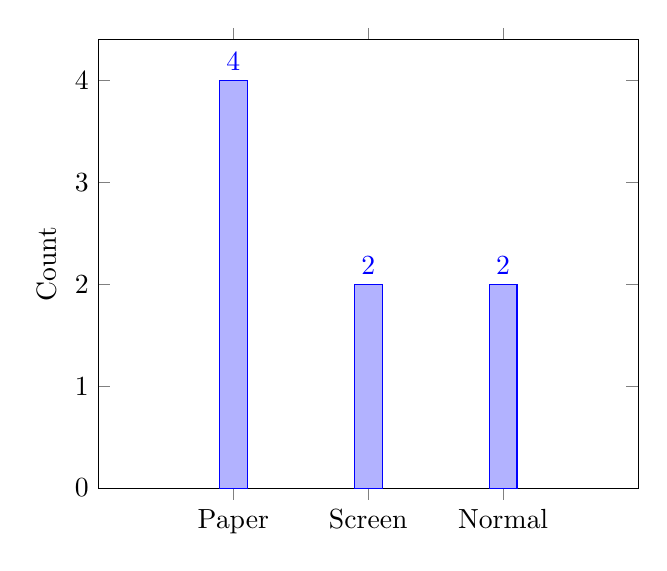
\begin{tikzpicture}
      \begin{axis}[
          ybar,
          ymin=0,
          enlarge x limits=0.5,
          legend style={at={(0.5,-0.15)},anchor=north,legend columns=-1},
          ylabel={Count},
          symbolic x coords={Paper, Screen, Normal},
          xtick=data,
          nodes near coords,
          ]
          \addplot coordinates {(Paper,4) (Screen,2) (Normal,2)};
      \end{axis}
    \end{tikzpicture}
    \label{fig:preference}
    \caption{System preference}
  \end{subfigure}
  ~
  \begin{subfigure}[t]{0.5\textwidth}
    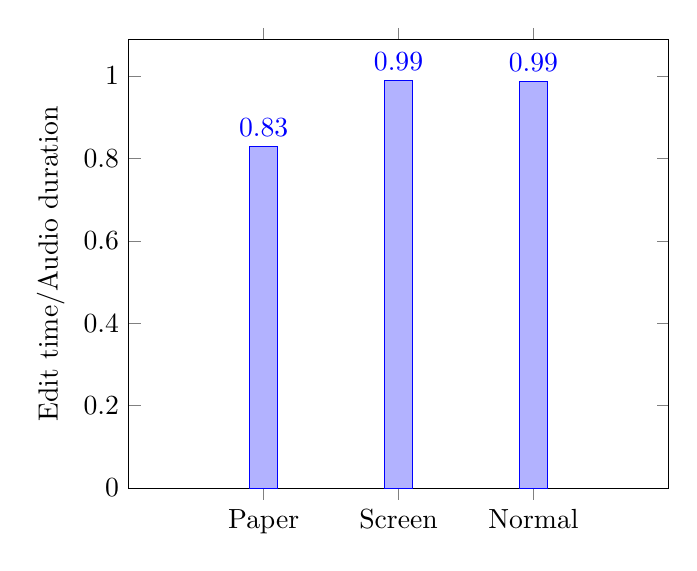
\begin{tikzpicture}
      \begin{axis}[
          ybar,
          ymin=0,
          enlarge x limits=0.5,
          legend style={at={(0.5,-0.15)},anchor=north,legend columns=-1},
          ylabel={Edit time/Audio duration},
          symbolic x coords={Paper, Screen, Normal},
          xtick=data,
          nodes near coords,
          ]
          \addplot coordinates {(Paper,0.8295) (Screen,0.9890) (Normal,0.9867)};
      \end{axis}
    \end{tikzpicture}
    \label{fig:paperspeed}
    \caption{Mean edit time, per minute of audio edited}
  \end{subfigure}
  \caption{Comparison of metrics}
\end{figure*}

\begin{itemize}
  \item Normal paper: 2
  \item Screen: 2
  \item Pen: 4
\end{itemize}

% Usefulness and usability
\subsubsection{Usefulness and usability}

\begin{figure}[h]
  \centering
	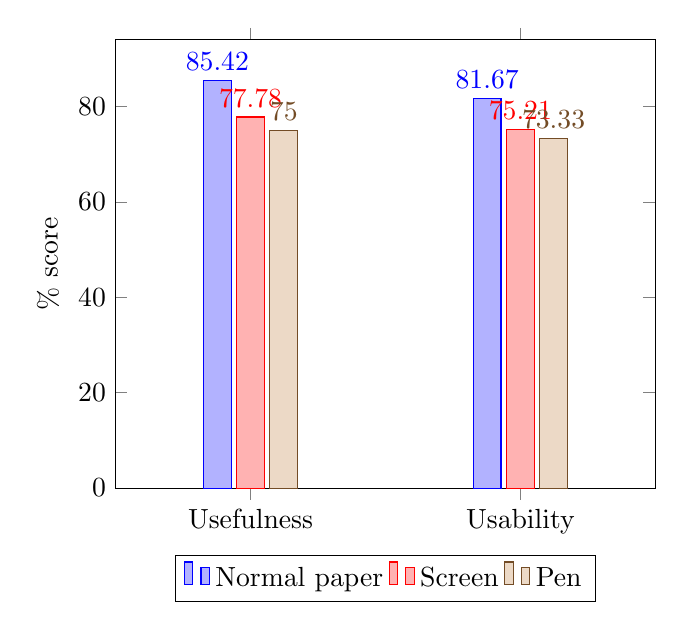
\begin{tikzpicture}
	\begin{axis}[
			ybar,
			ymin=0,
			enlarge x limits=0.5,
			legend style={at={(0.5,-0.15)},anchor=north,legend columns=-1},
			ylabel={\% score},
			symbolic x coords={Usefulness, Usability},
			xtick=data,
			nodes near coords,
			nodes near coords align={vertical},
			]
	\addplot coordinates {(Usefulness,85.42) (Usability,81.67)};
	\addplot coordinates {(Usefulness,77.78) (Usability,75.21)};
	\addplot coordinates {(Usefulness,75.00) (Usability,73.33)};
	\legend{Normal paper, Screen, Pen}
	\end{axis}
	\end{tikzpicture}
  \label{fig:usefulusable}
  \caption{Mean average scores for usefulness and usability}
\end{figure}


% Speed
\subsubsection{Speed}

\begin{figure}[h]
  \centering
  \begin{tikzpicture}
  \begin{axis}[
    legend pos=outer north east,
    legend cell align=left,
    xmin=0,
    ymin=0,
    xlabel={Audio length (mins)},
    ylabel={Edit time (mins)}]

  % NORMAL
  \pgfplotstableread{
    X Y
    30 30
    58 43
    32 23
    35 53
    28 35
    28 32
    47 62
    28 22
  }\normaltimes
  \addplot [only marks, mark = *, red] table {\normaltimes};
  \addlegendentry{Normal paper}
  \addplot [thick, red, forget plot] table[
      y={create col/linear regression={y=Y}}
  ]{\normaltimes};
  %\addlegendentry{Normal trend}

  % SCREEN
  \pgfplotstableread{
    X Y
    37 24
    61 61
    30 30
    25 49
    26 31
    41 28
    37 37
    33 45
  }\screentimes
  \addplot [only marks, mark = square*, blue] table {\screentimes};
  \addlegendentry{Screen}
  \addplot [thick, dotted, blue, forget plot] table[
      y={create col/linear regression={y=Y}}
  ]{\screentimes};
  %\addlegendentry{Screen trend}

  % PEN
  \pgfplotstableread{
    X Y
    12 9
    75 56
    31 17
    22 19
    27 27
    38 37
    33 33
    28 41
  }\pentimes
  \addplot [only marks, mark = diamond*, green] table {\pentimes};
  \addlegendentry{Pen}
  \addplot [thick, loosely dashed, green, forget plot] table[
      y={create col/linear regression={y=Y}}
  ]{\pentimes};
  %\addlegendentry{Pen trend}

  \end{axis}
  \end{tikzpicture}
  \caption{Edit time performance for each editing system, with linear regression plot}
  \label{fig:penedittime}
\end{figure}

Mean edit time, per minute of input audio:
\begin{itemize}
    \item Normal paper: 59.2 seconds (x0.9867 real-time)
    \item Screen: 59.34 seconds (x0.9890 real-time)
    \item Pen: 49.77 seconds (x0.8295 real-time)
\end{itemize}

% Usefulness


% Usability




\section{Discussion}\label{sec:paper-discussion}

% Paper better for solo working
% - notes don't have to be digitised/shared

% Screen better for collaboration
% - can be done remotely
% - annotations are digital, interface can be updated


\section{Conclusion}\label{sec:paper-conclusion}

\subsection{Future work}
